% You should title the file with a .tex extension (hw1.tex, for example)
\documentclass[11pt]{article}

\usepackage{amsmath}
\usepackage{mathtools}
\usepackage{amssymb}
\usepackage{fancyhdr}
\usepackage{tikz-qtree}
\usepackage{tikz-qtree-compat}
\usepackage[normalem]{ulem}
\usepackage{tikz}
\usepackage{graphicx}
\DeclareMathOperator*{\argmin}{argmin}
\DeclareMathOperator*{\argmax}{argmax}

\oddsidemargin0cm
\topmargin-2cm     %I recommend adding these three lines to increase the 
\textwidth16.5cm   %amount of usable space on the page (and save trees)
\textheight23.5cm  

\newcommand{\question}[2] {\vspace{.25in} \hrule\vspace{0.5em}
\noindent{\bf #1: #2} \vspace{0.5em}
\hrule \vspace{.10in}}
\renewcommand{\part}[1] {\vspace{.10in} {\bf (#1)}}

\newcommand{\myname}{Sean Bittner}
\newcommand{\myandrew}{srb2201@columbia.edu}
\newcommand{\myhwnum}{12}

\setlength{\parindent}{0pt}
\setlength{\parskip}{5pt plus 1pt}
 
\DeclarePairedDelimiter\abs{\lvert}{\rvert}%
 
\pagestyle{fancyplain}
\rhead{\fancyplain{}{\myname\\ \myandrew}}

\begin{document}

\medskip                        % Skip a "medium" amount of space
                                % (latex determines what medium is)
                                % Also try: \bigskip, \littleskip

\thispagestyle{plain}
\begin{center}                  % Center the following lines
{\Large Linear 2D system oscillation DSN} \\
Aug 19, 2018 \\
\end{center}
\question{1}{2D linear system with oscillations}
We're considering the 2D linear system
\[\tau \dot{x} = -x + Wx\]
\[W = \begin{bmatrix} w_1 & w_2 \\ w_3 & w_4 \end{bmatrix} \]
Where the linear dynamics can characterized by an eigendecomposition of the linear dynamics matrix
\[\dot{x} = Ax, A = \frac{1}{\tau}(W-I) = \begin{bmatrix} a_1 & a_2 \\ a_3 & a_4 \end{bmatrix} \]

If we want to learn a gaussian distribution of pure oscillations, the eigenvalues of A (and W) should have zero real part, and the imaginary components should be complex conjugate pairs with magnitude corresponding to the desired frequency.  The behavior I imposed on this 2D linear system DSN was:
\[ E[T(g(\phi))] = \begin{bmatrix} real(\lambda_1)\\ real(\lambda_1)^2 \\  real(\lambda_2)\\ real(\lambda_2)^2 \\  imag(\lambda_1)\\ imag(\lambda_1)^2 \end{bmatrix}  = \begin{bmatrix} 0.0 \\ 0.001 \\ 0.0 \\ 0.001 \\ 16.0 \\ 0.1 \end{bmatrix} \]

I trained DSN's to learn the space of real entries of both A (section 2) and W (section3, $\tau = 100ms$).  I tested 5 architectures: \\
1A - one affine transformation \\
2P - two planar flows (two nonlinear normalizing flows) \\
4P, 8P, ... \\
10P - ten planar flows  \\

For each architecture I tested three different initializations of the augmented lagrangian optimization paramter $c \in \left[ 10^{-5}, 1, 10^5 \right]$, and three separate learning rates $lr \in \left[ 10^{-4}, 10^{-3}, 10^{-2} \right]$


\clearpage

\question{2}{Learning A}
\begin{center}
\textbf{1 affine layer} \\
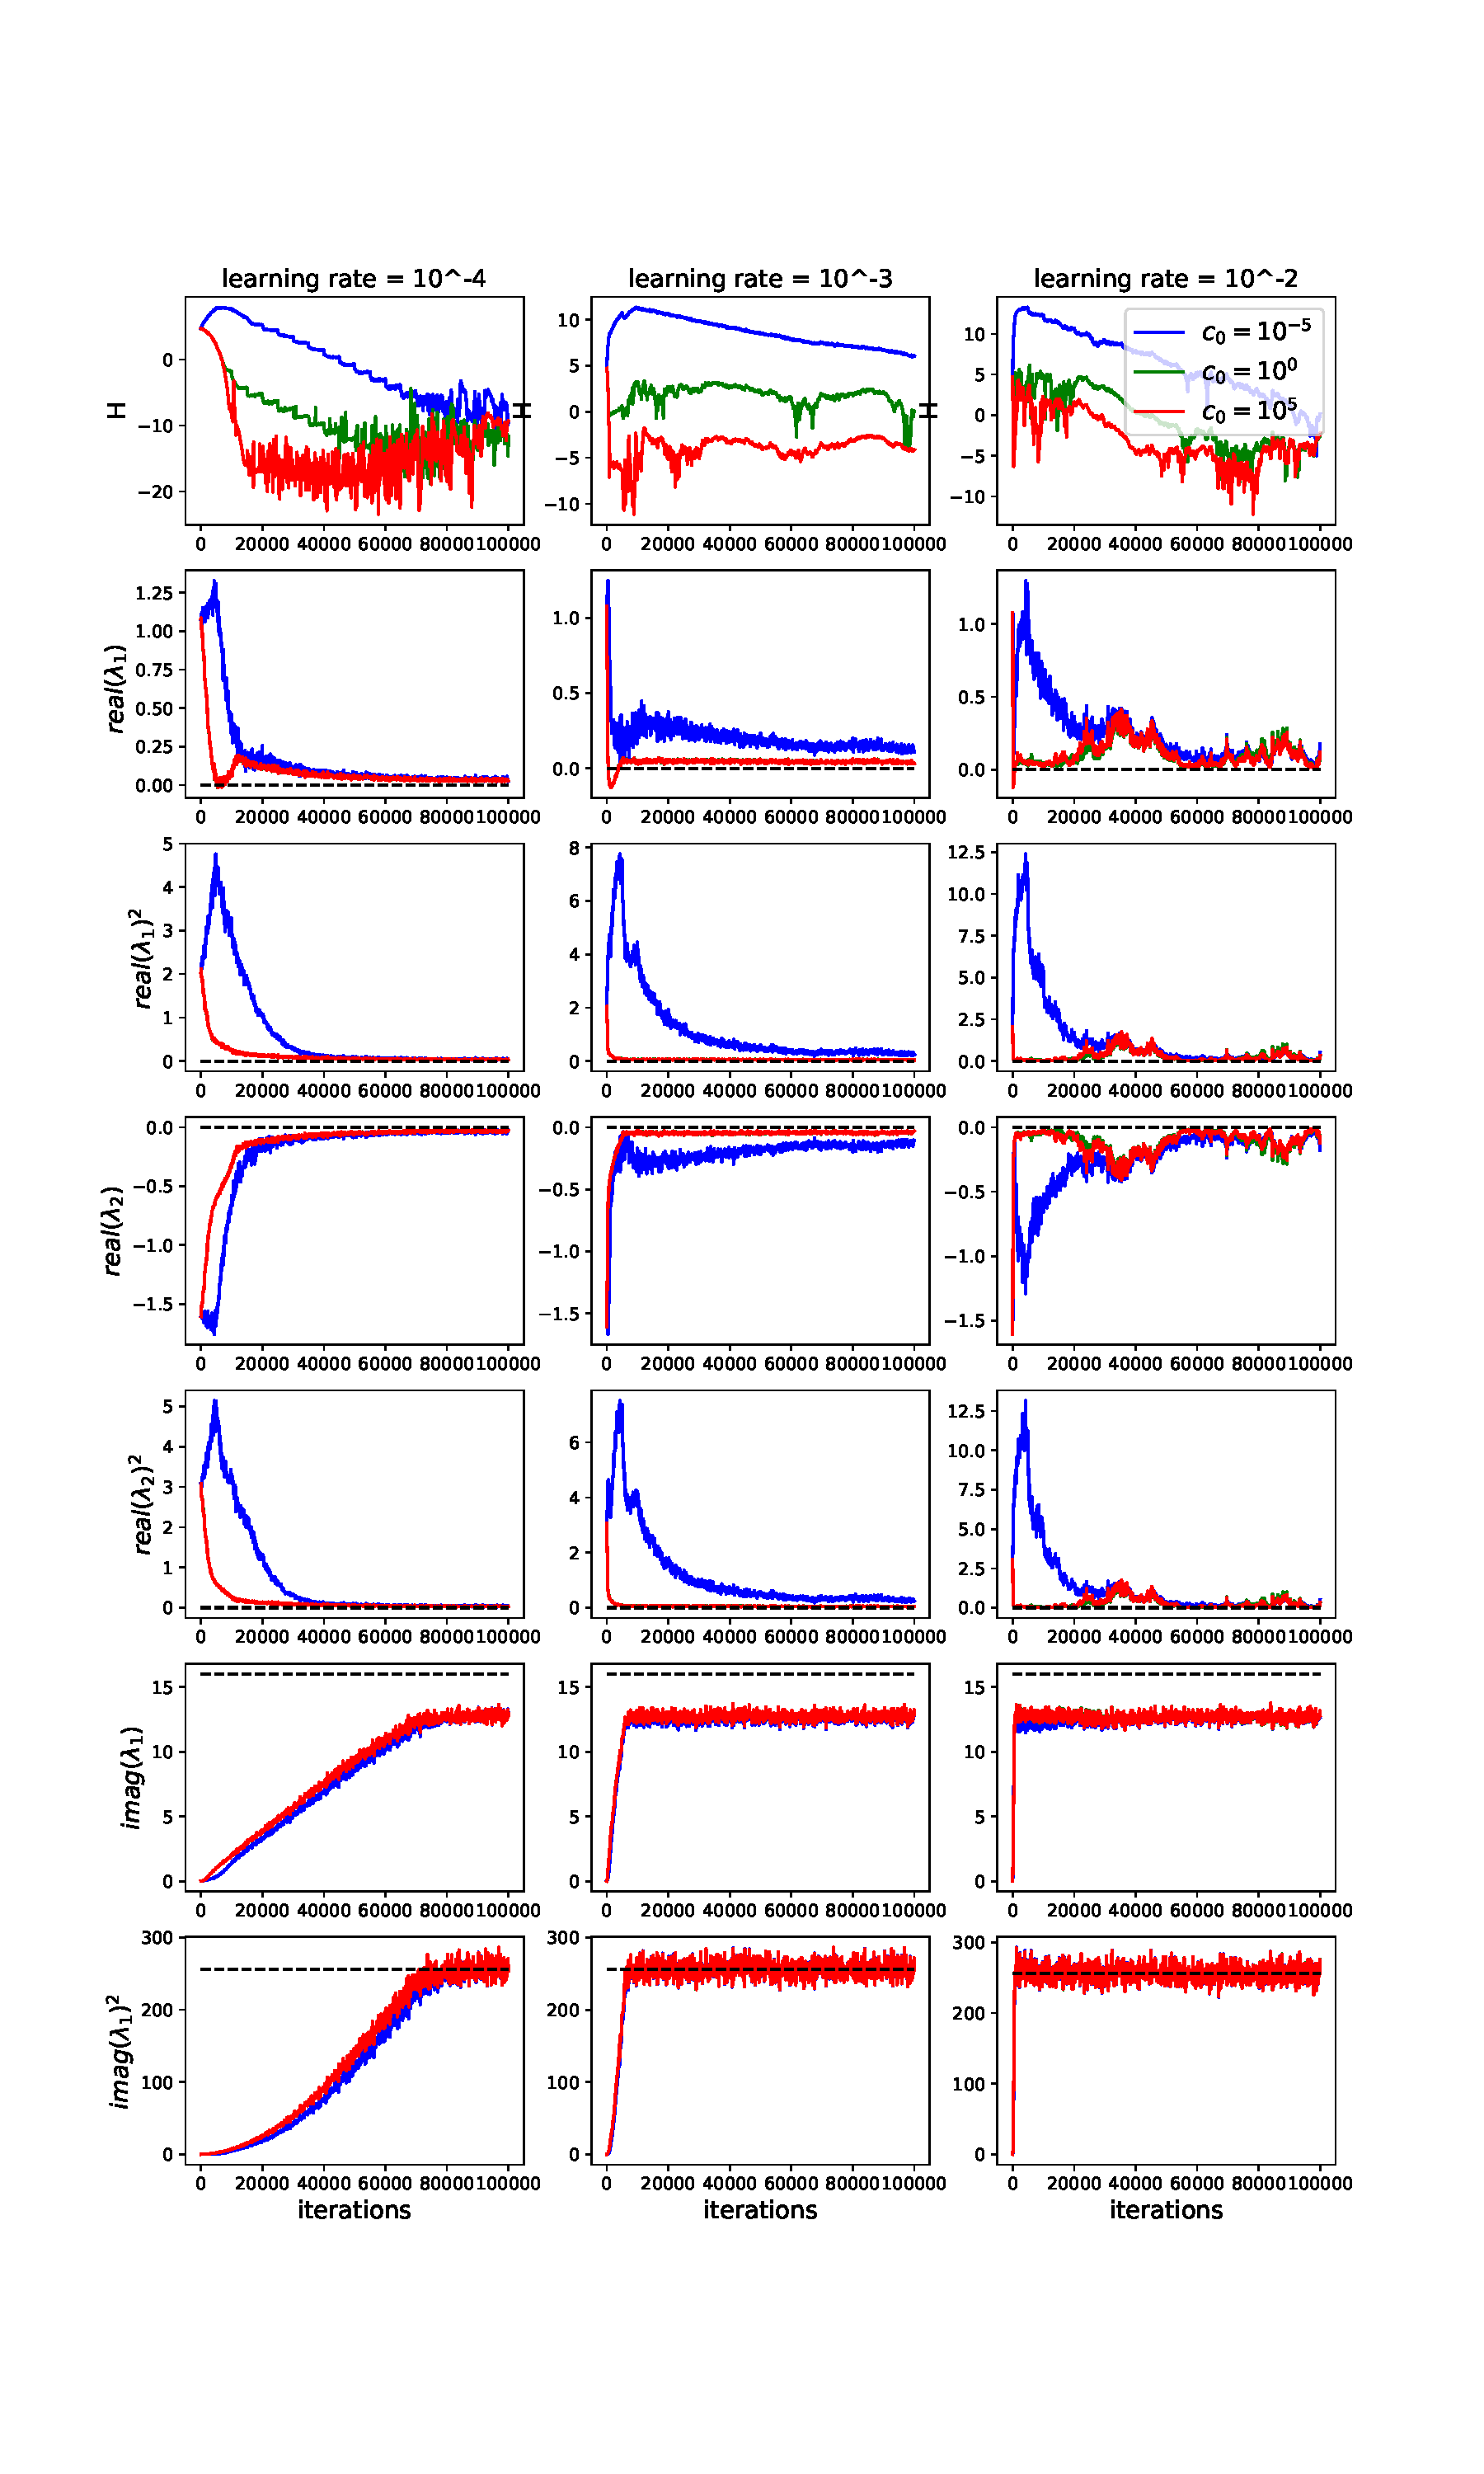
\includegraphics[scale=.41]{images/learnA_1A.pdf} \\
\end{center}

\clearpage
\begin{center}
\textbf{2 planar layers} \\
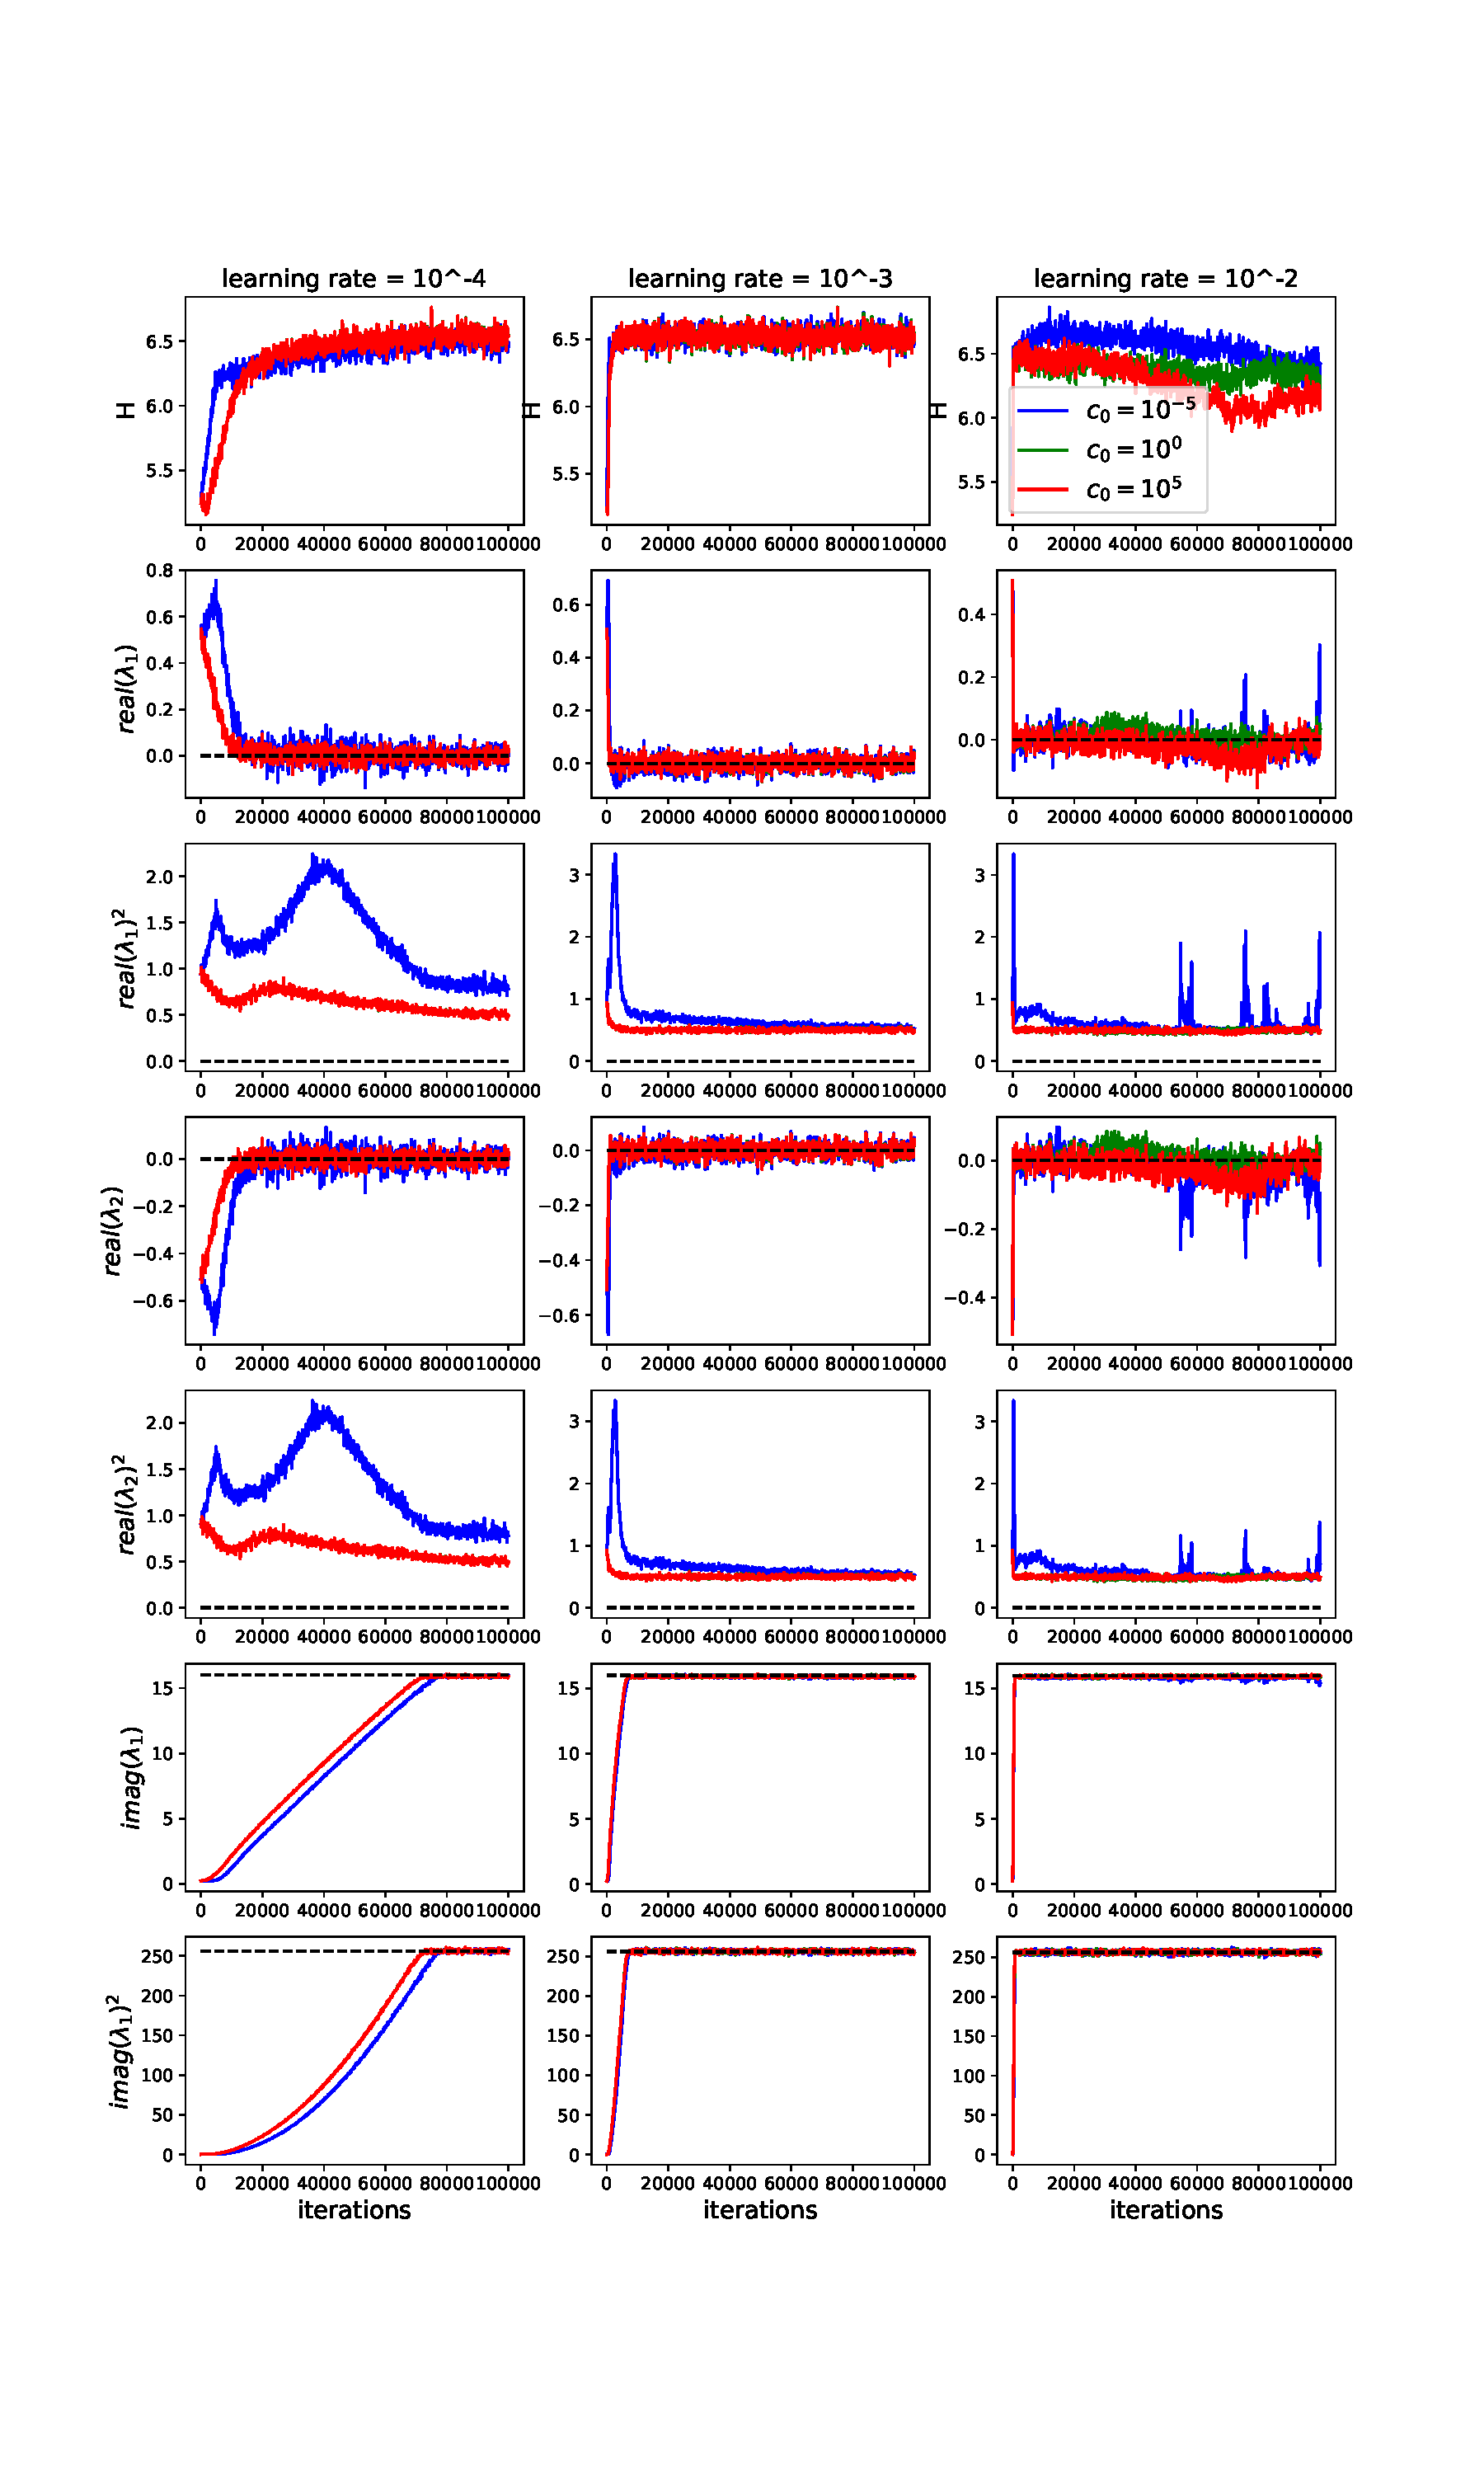
\includegraphics[scale=.45]{images/learnA_2P.pdf} \\
\end{center}

\clearpage
\begin{center}
\textbf{4 planar layers} \\
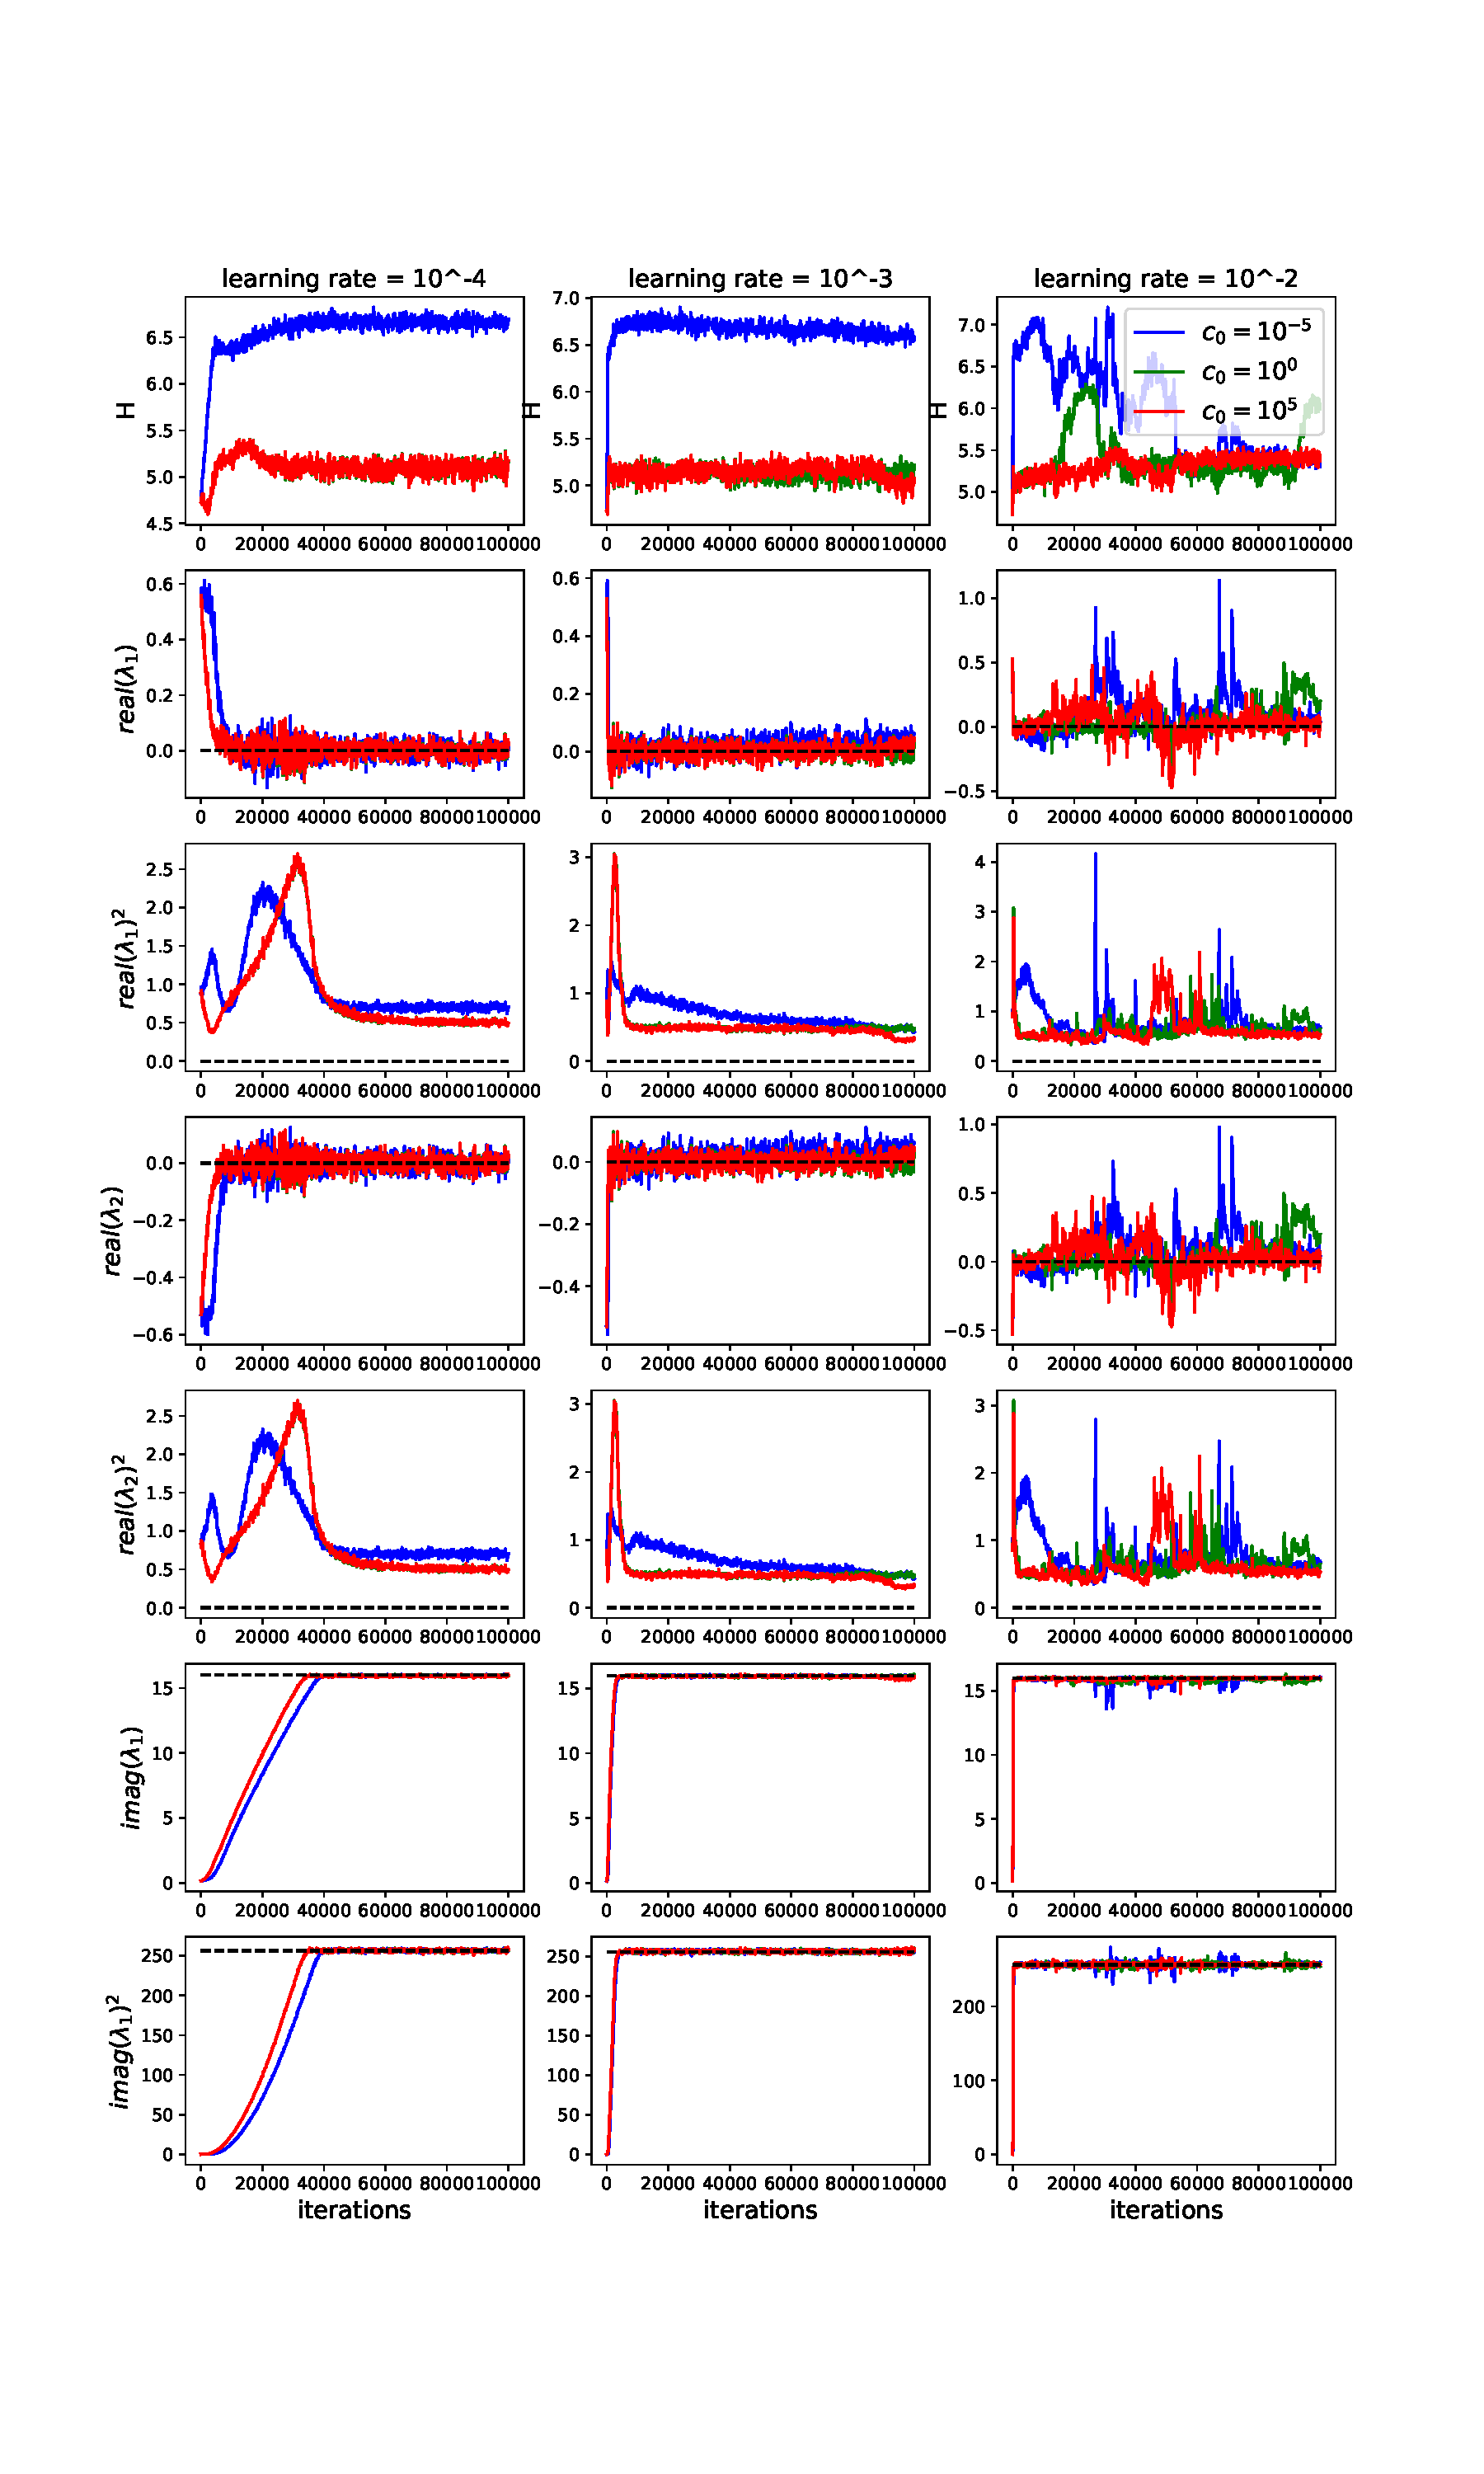
\includegraphics[scale=.45]{images/learnA_4P.pdf} \\
\end{center}

\clearpage
\begin{center}
\textbf{8 planar layers} \\
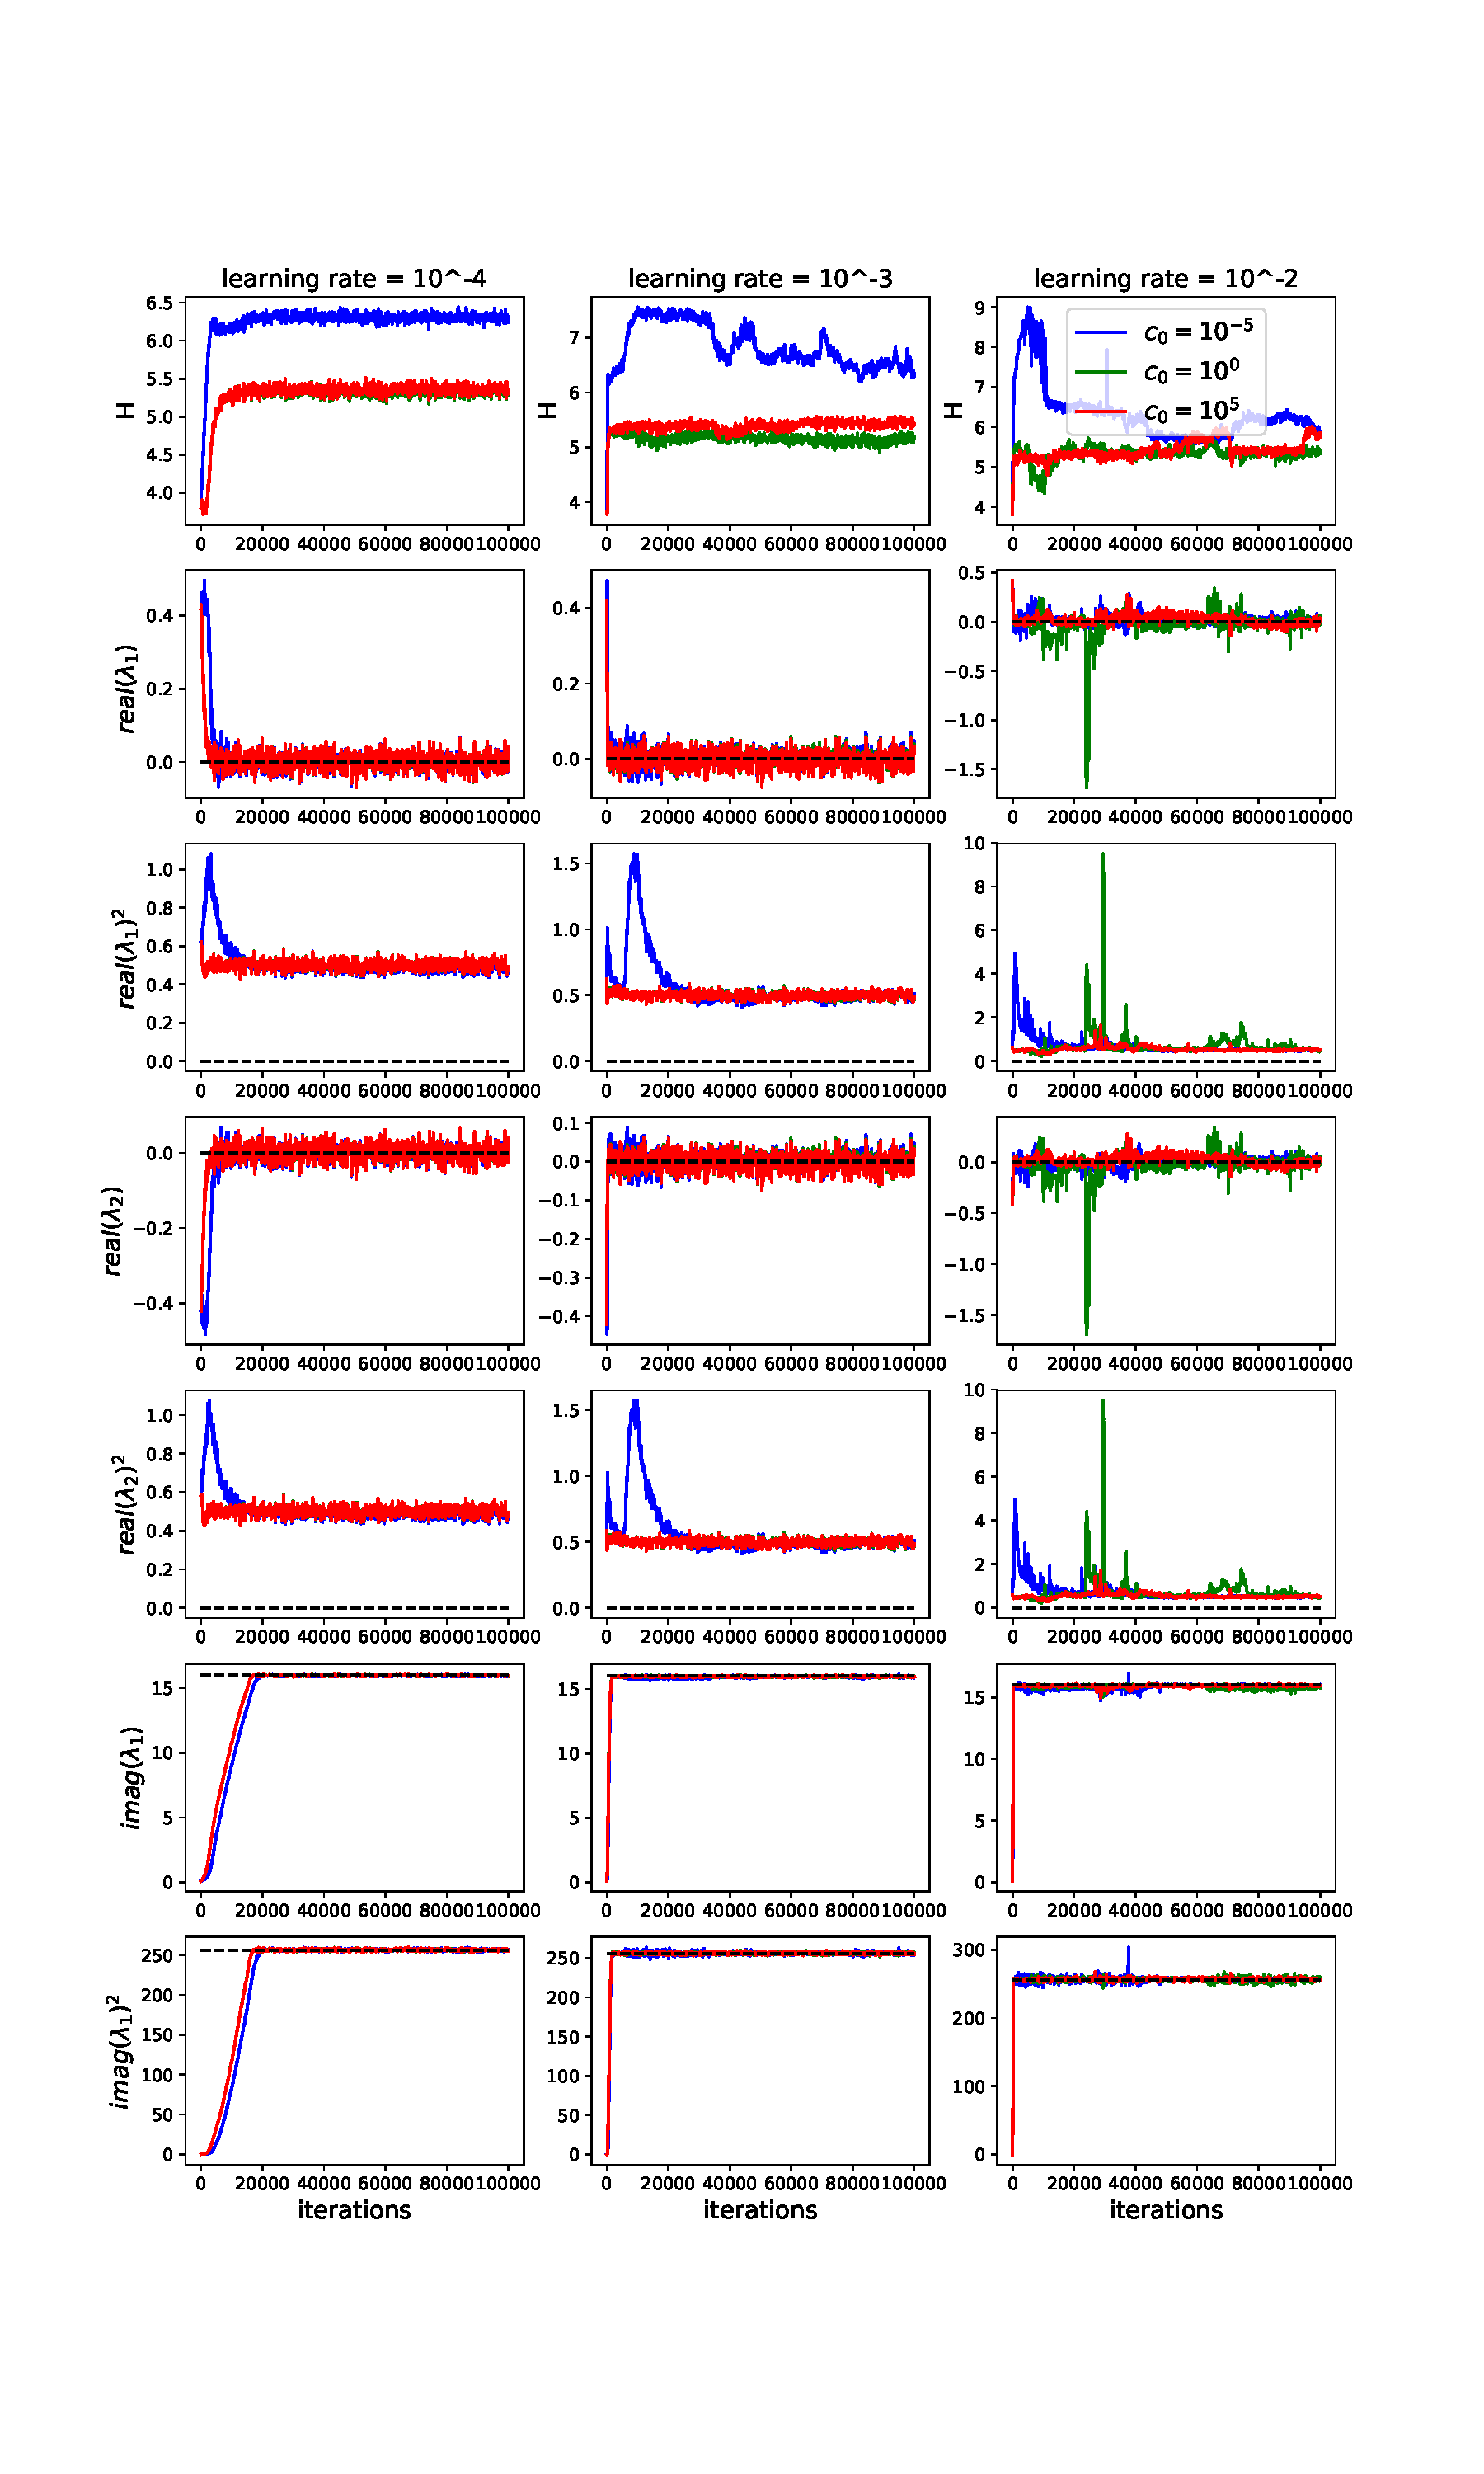
\includegraphics[scale=.45]{images/learnA_8P.pdf} \\
\end{center}

\clearpage
\begin{center}
\textbf{10 planar layers} \\
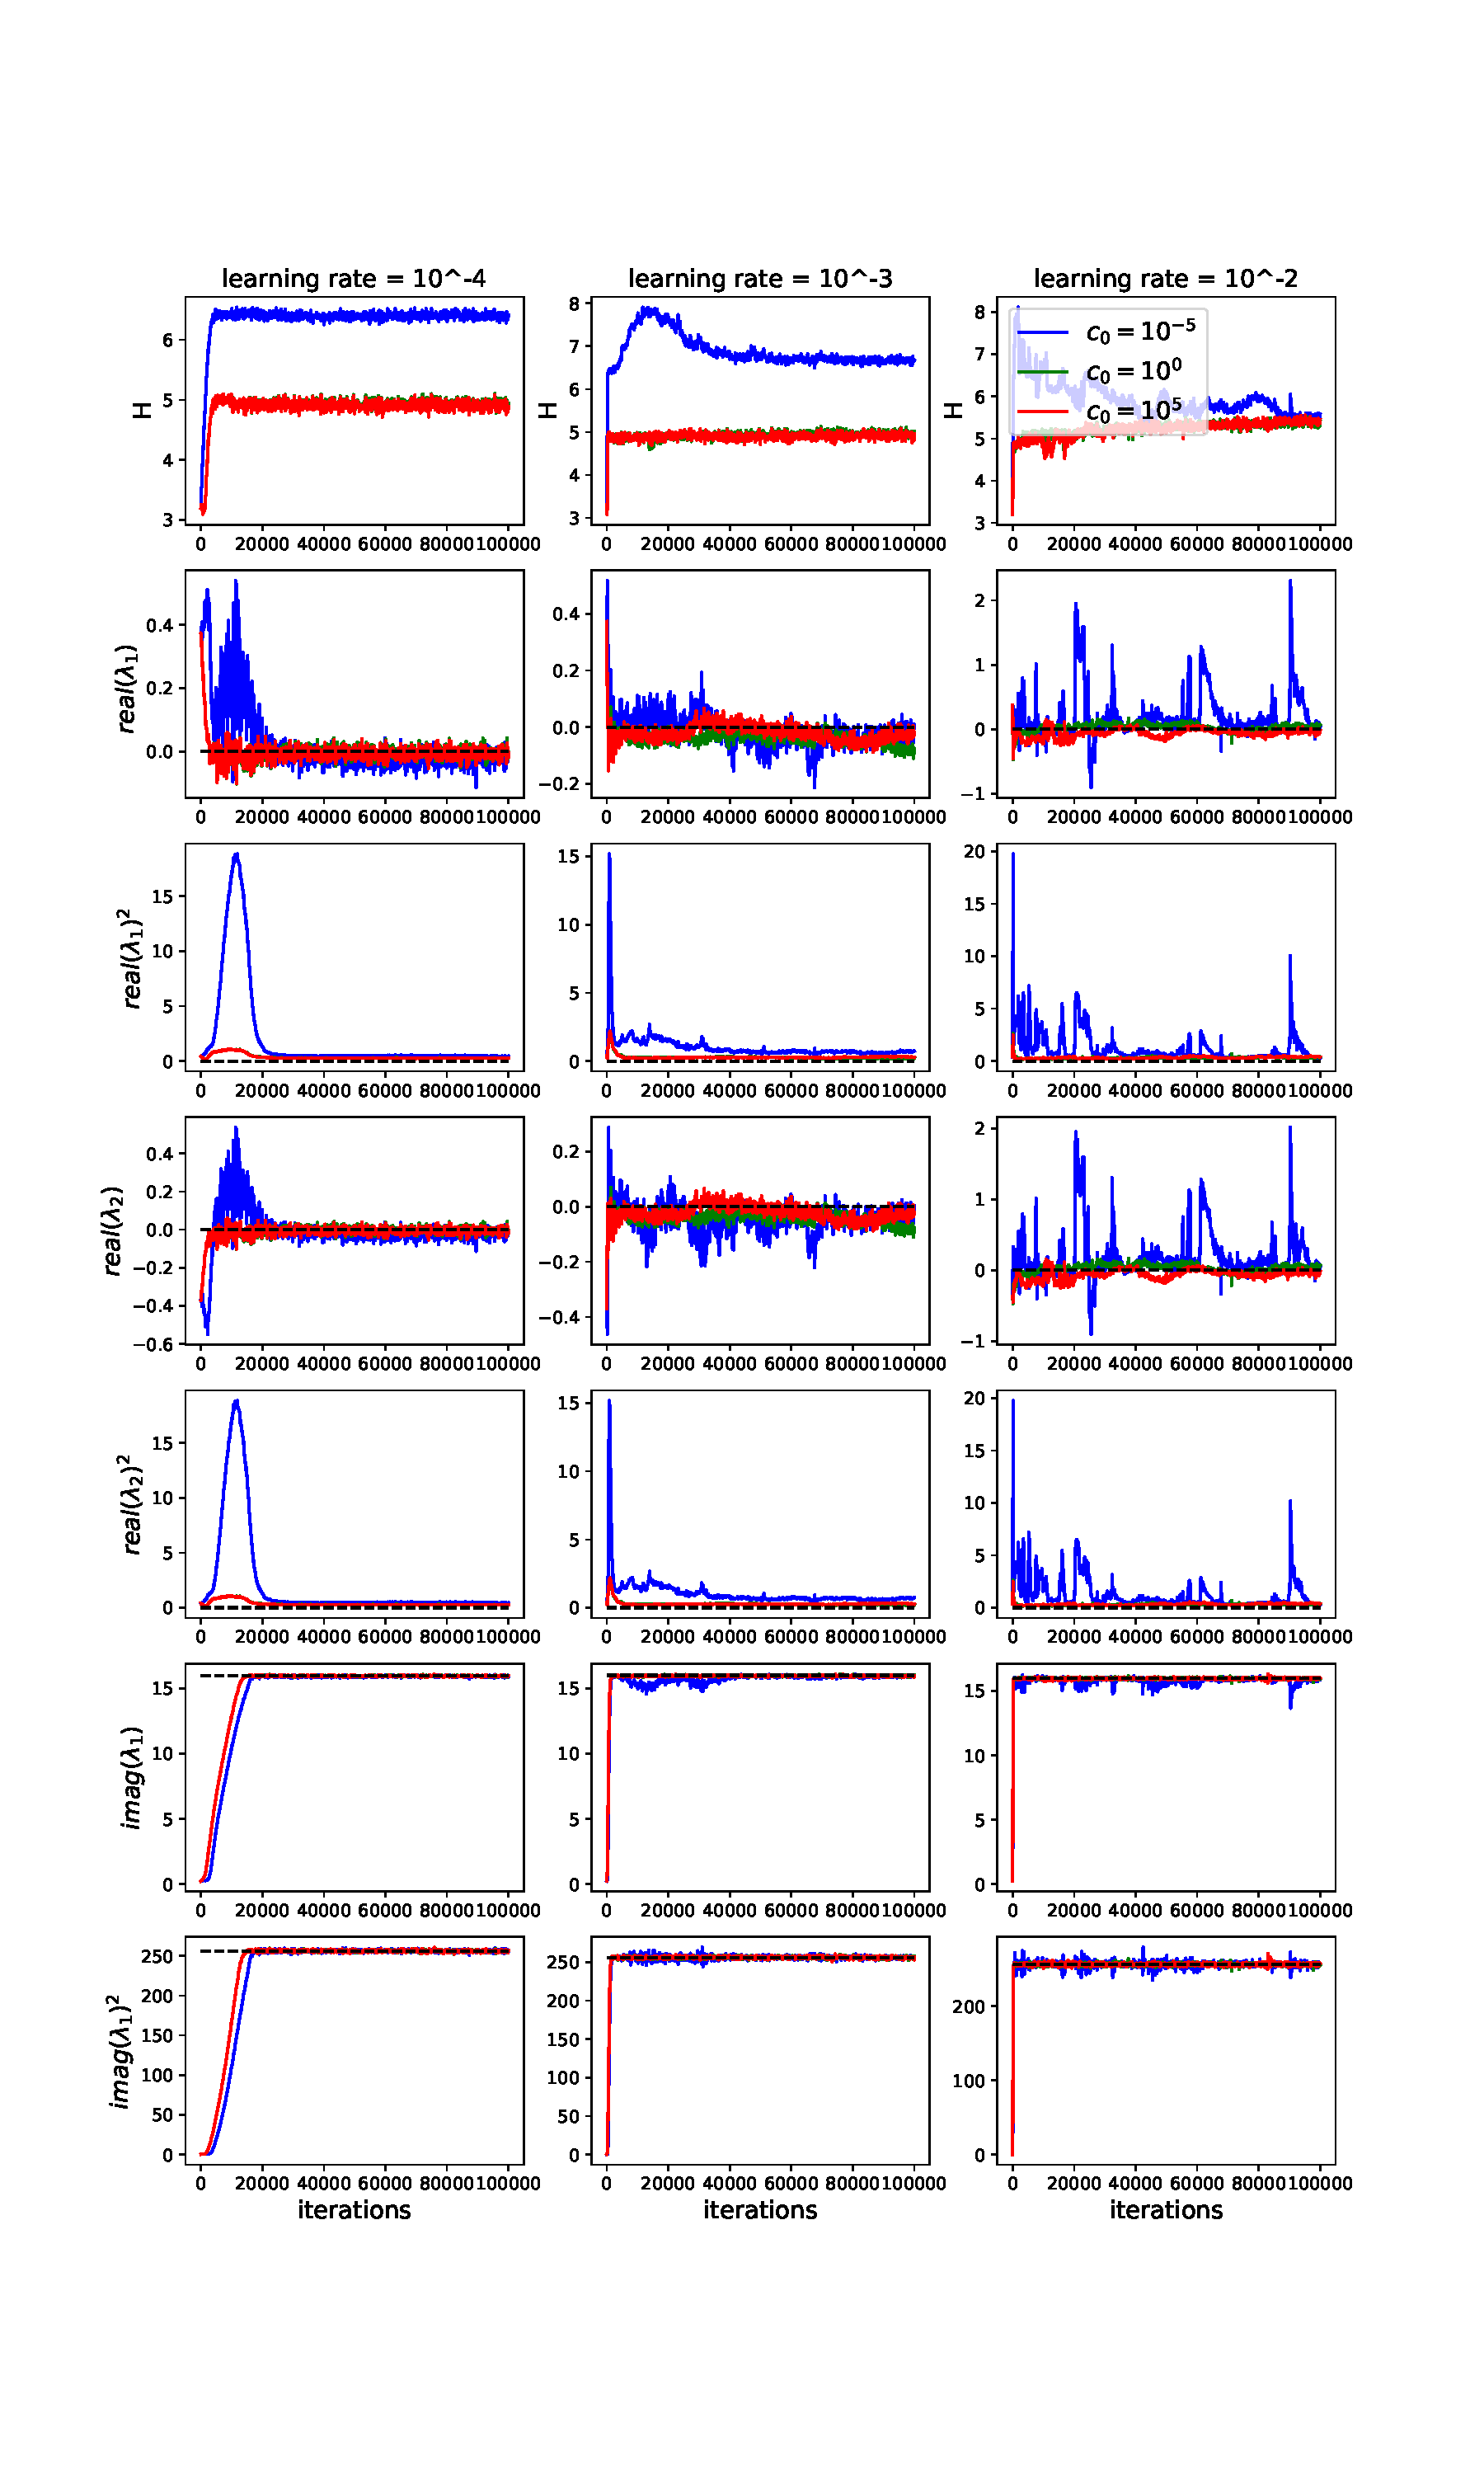
\includegraphics[scale=.45]{images/learnA_10P.pdf} \\
\end{center}

\clearpage
\begin{center}
\textbf{A: 10 planar layers}: $c_0 = 1$, learning rate = $10^{-3}$ \\
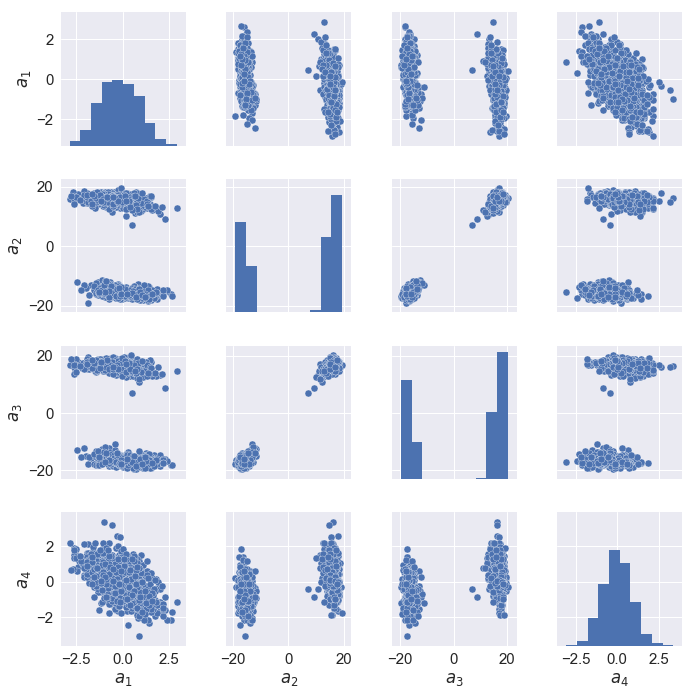
\includegraphics[scale=.45]{images/learnA_samples.png} \\
\end{center}
\clearpage



\question{3}{Learning W}
\begin{center}
\textbf{W: 1 affine layer} \\
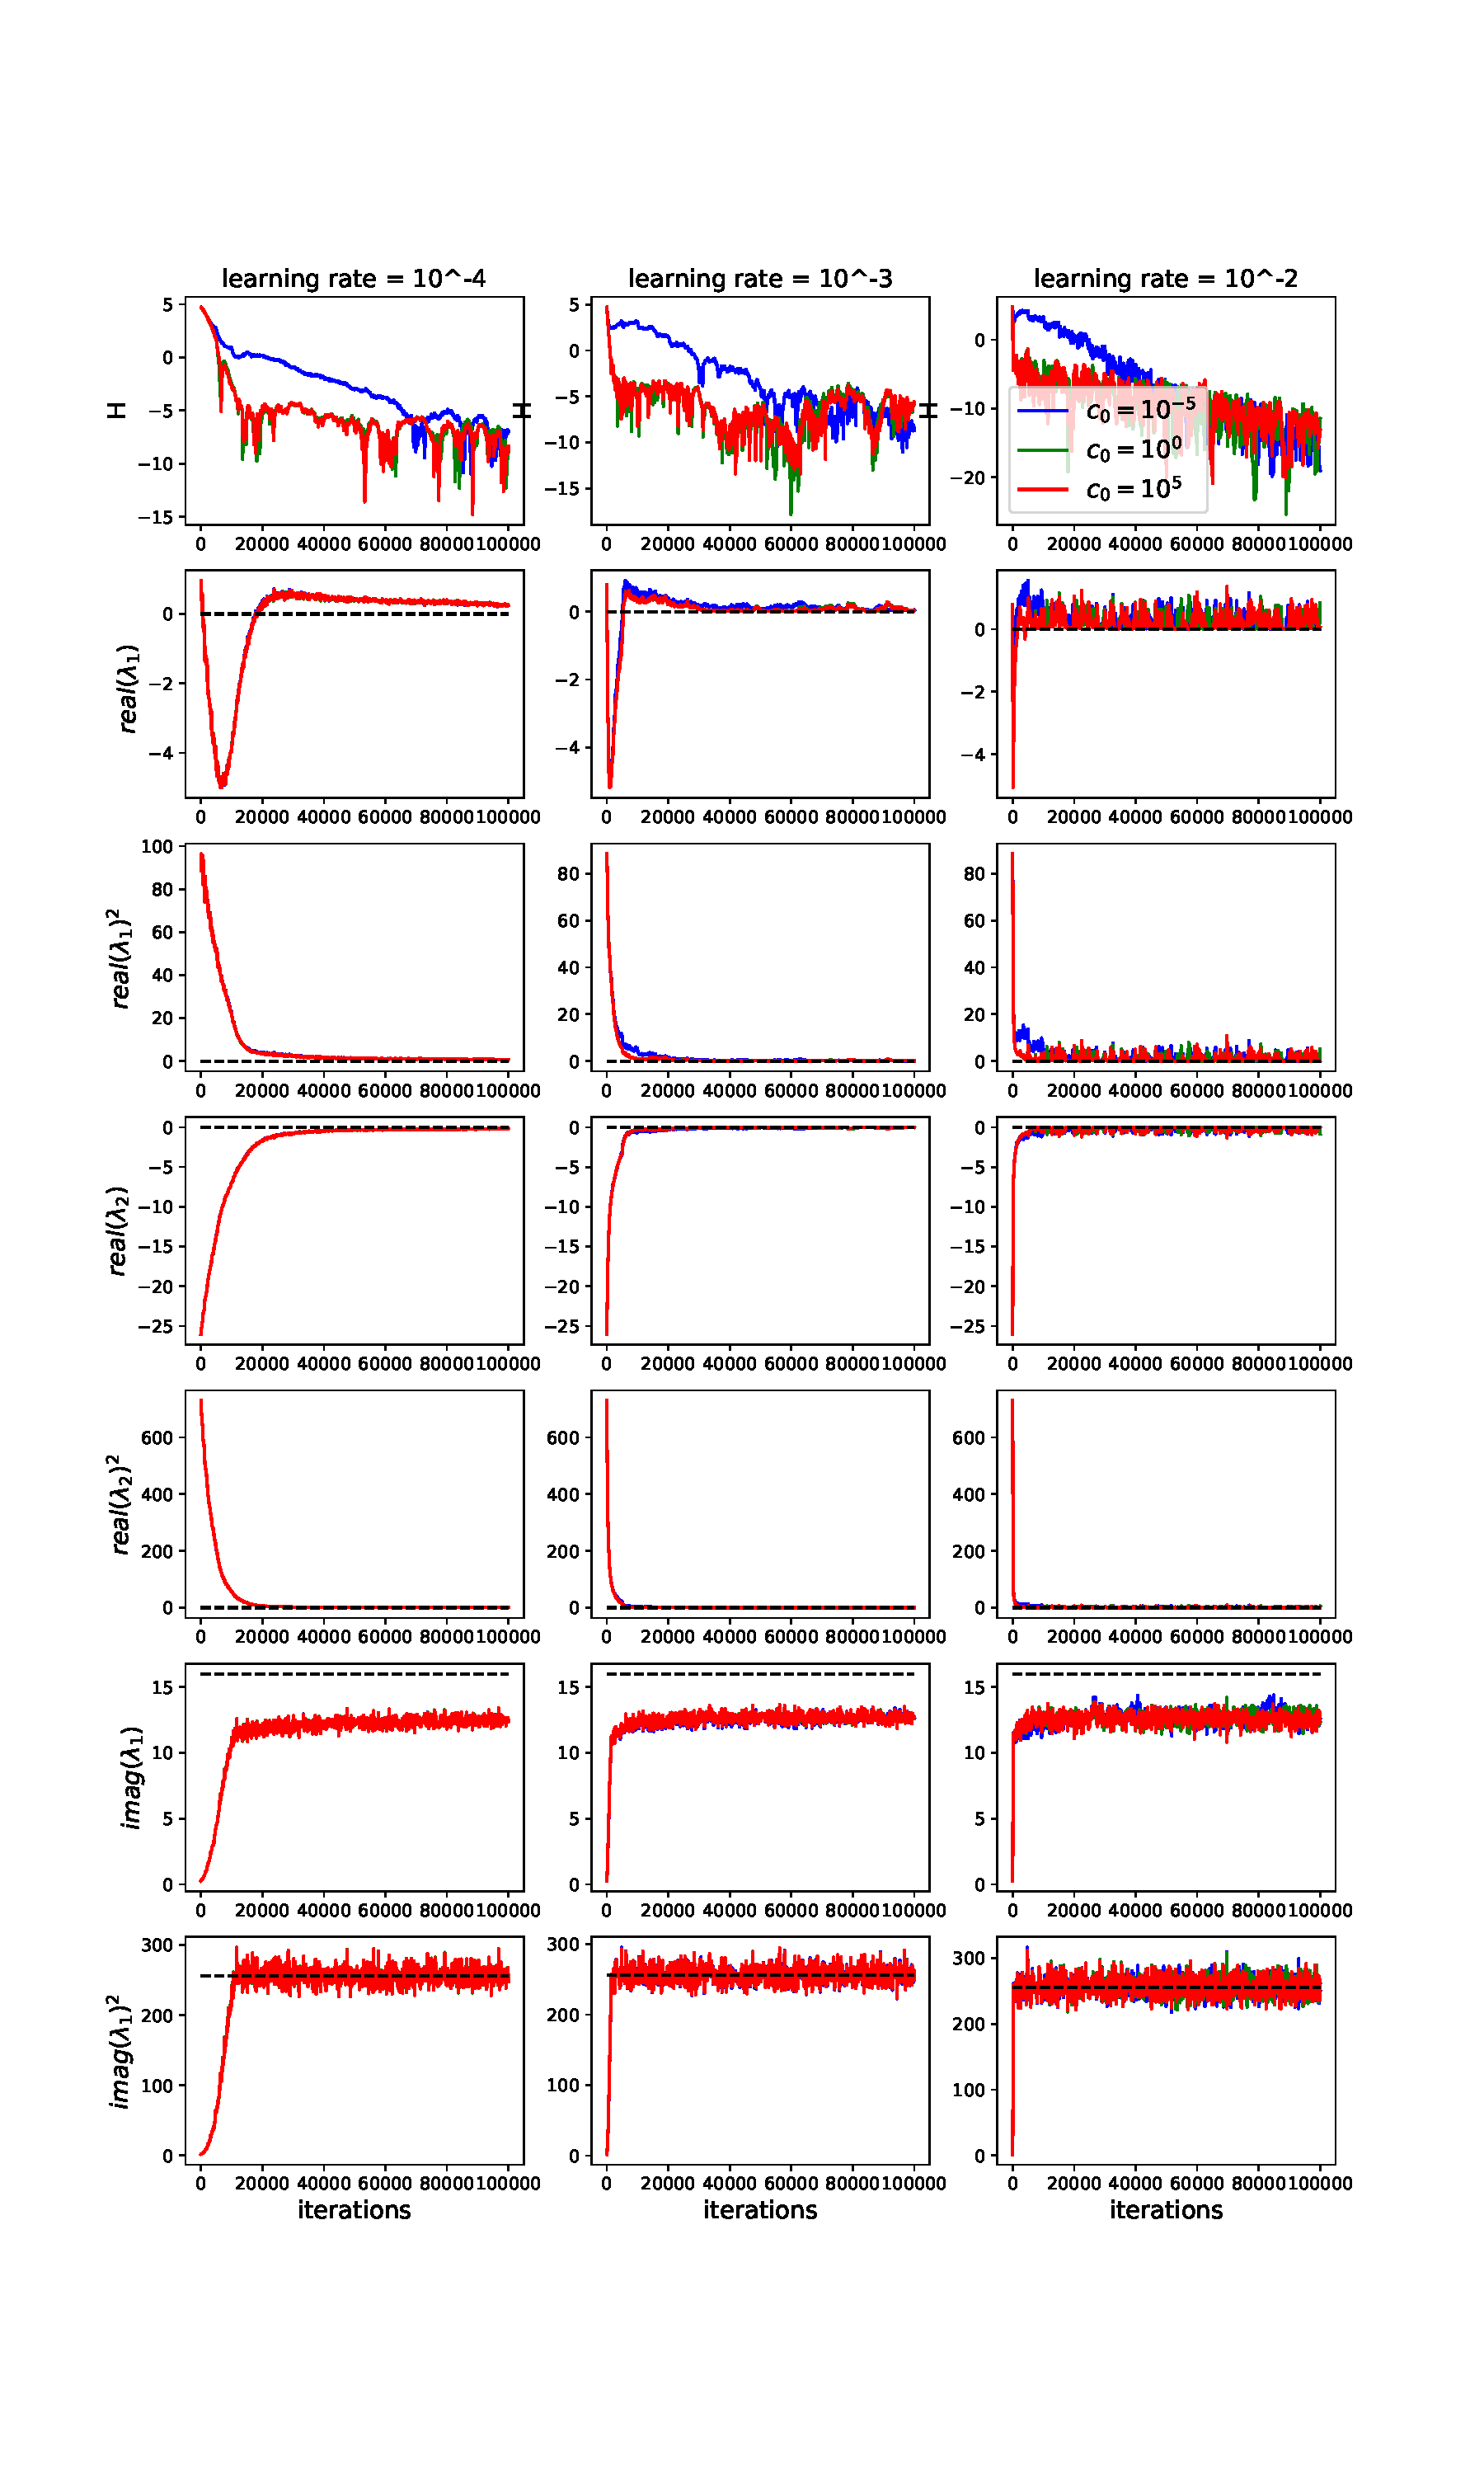
\includegraphics[scale=.41]{images/learnW_1A.pdf} \\
\end{center}

\clearpage
\begin{center}
\textbf{W: 2 planar layers} \\
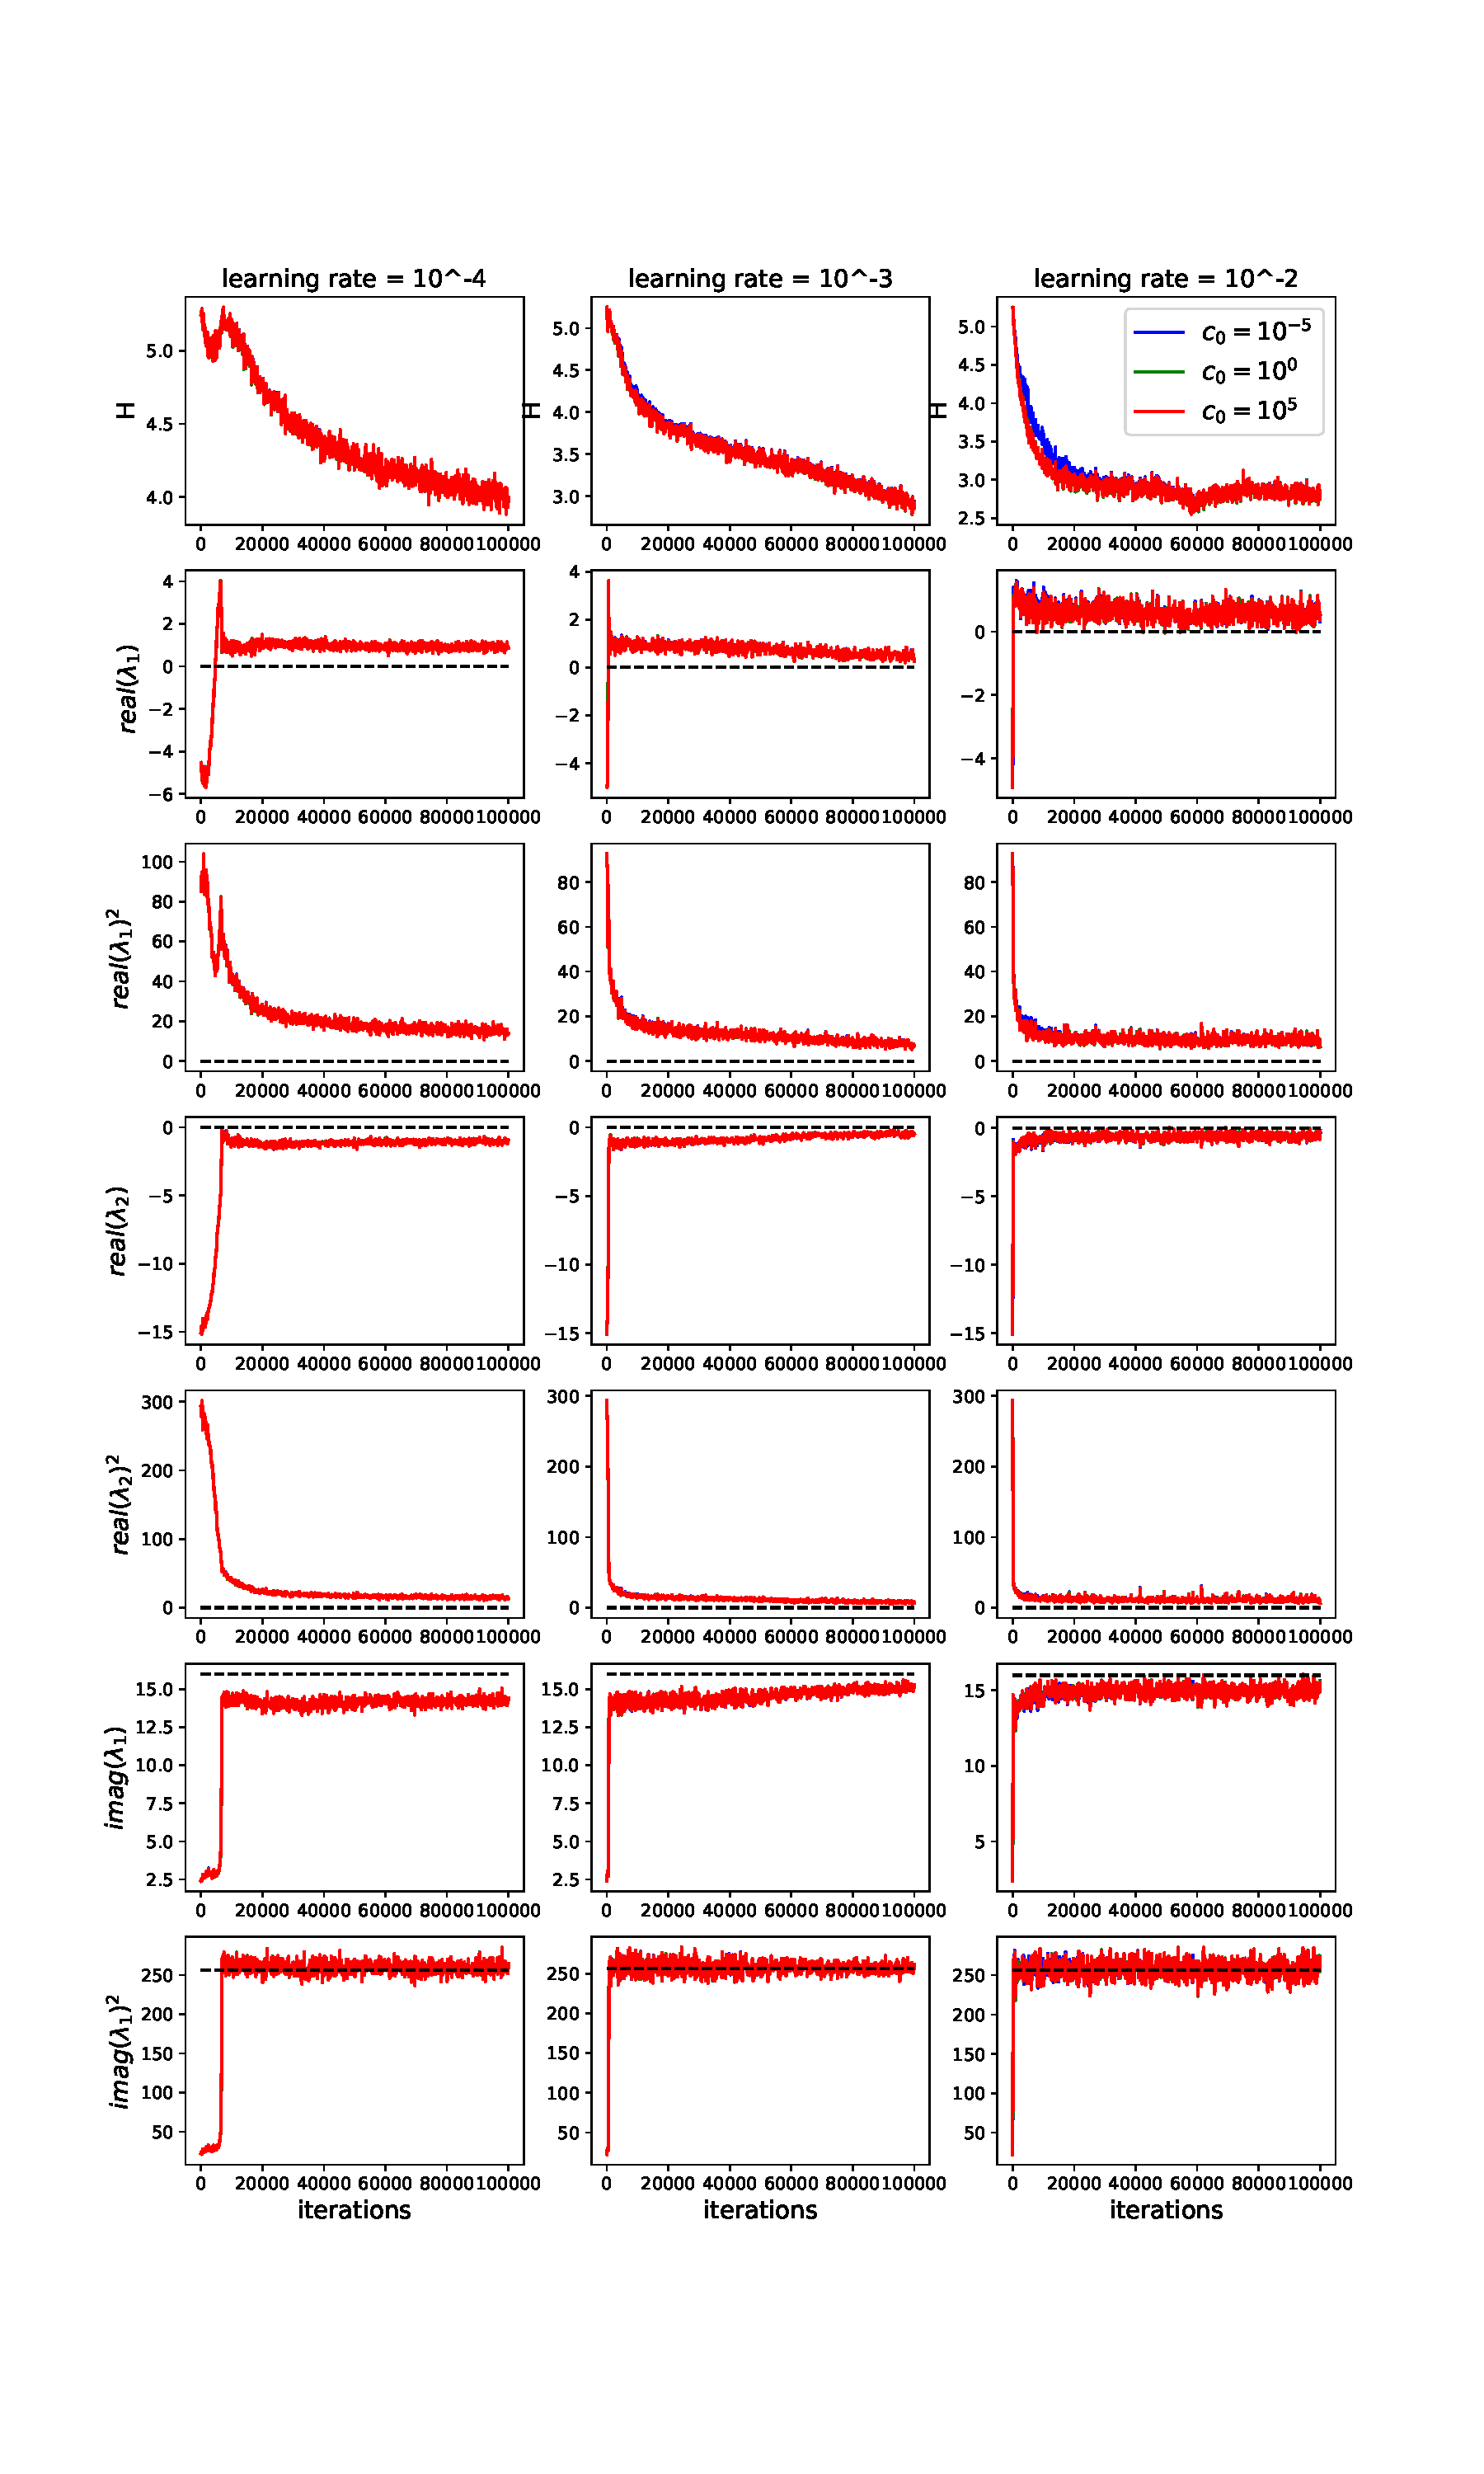
\includegraphics[scale=.45]{images/learnW_2P.pdf} \\
\end{center}

\clearpage
\begin{center}
\textbf{W: 4 planar layers} \\
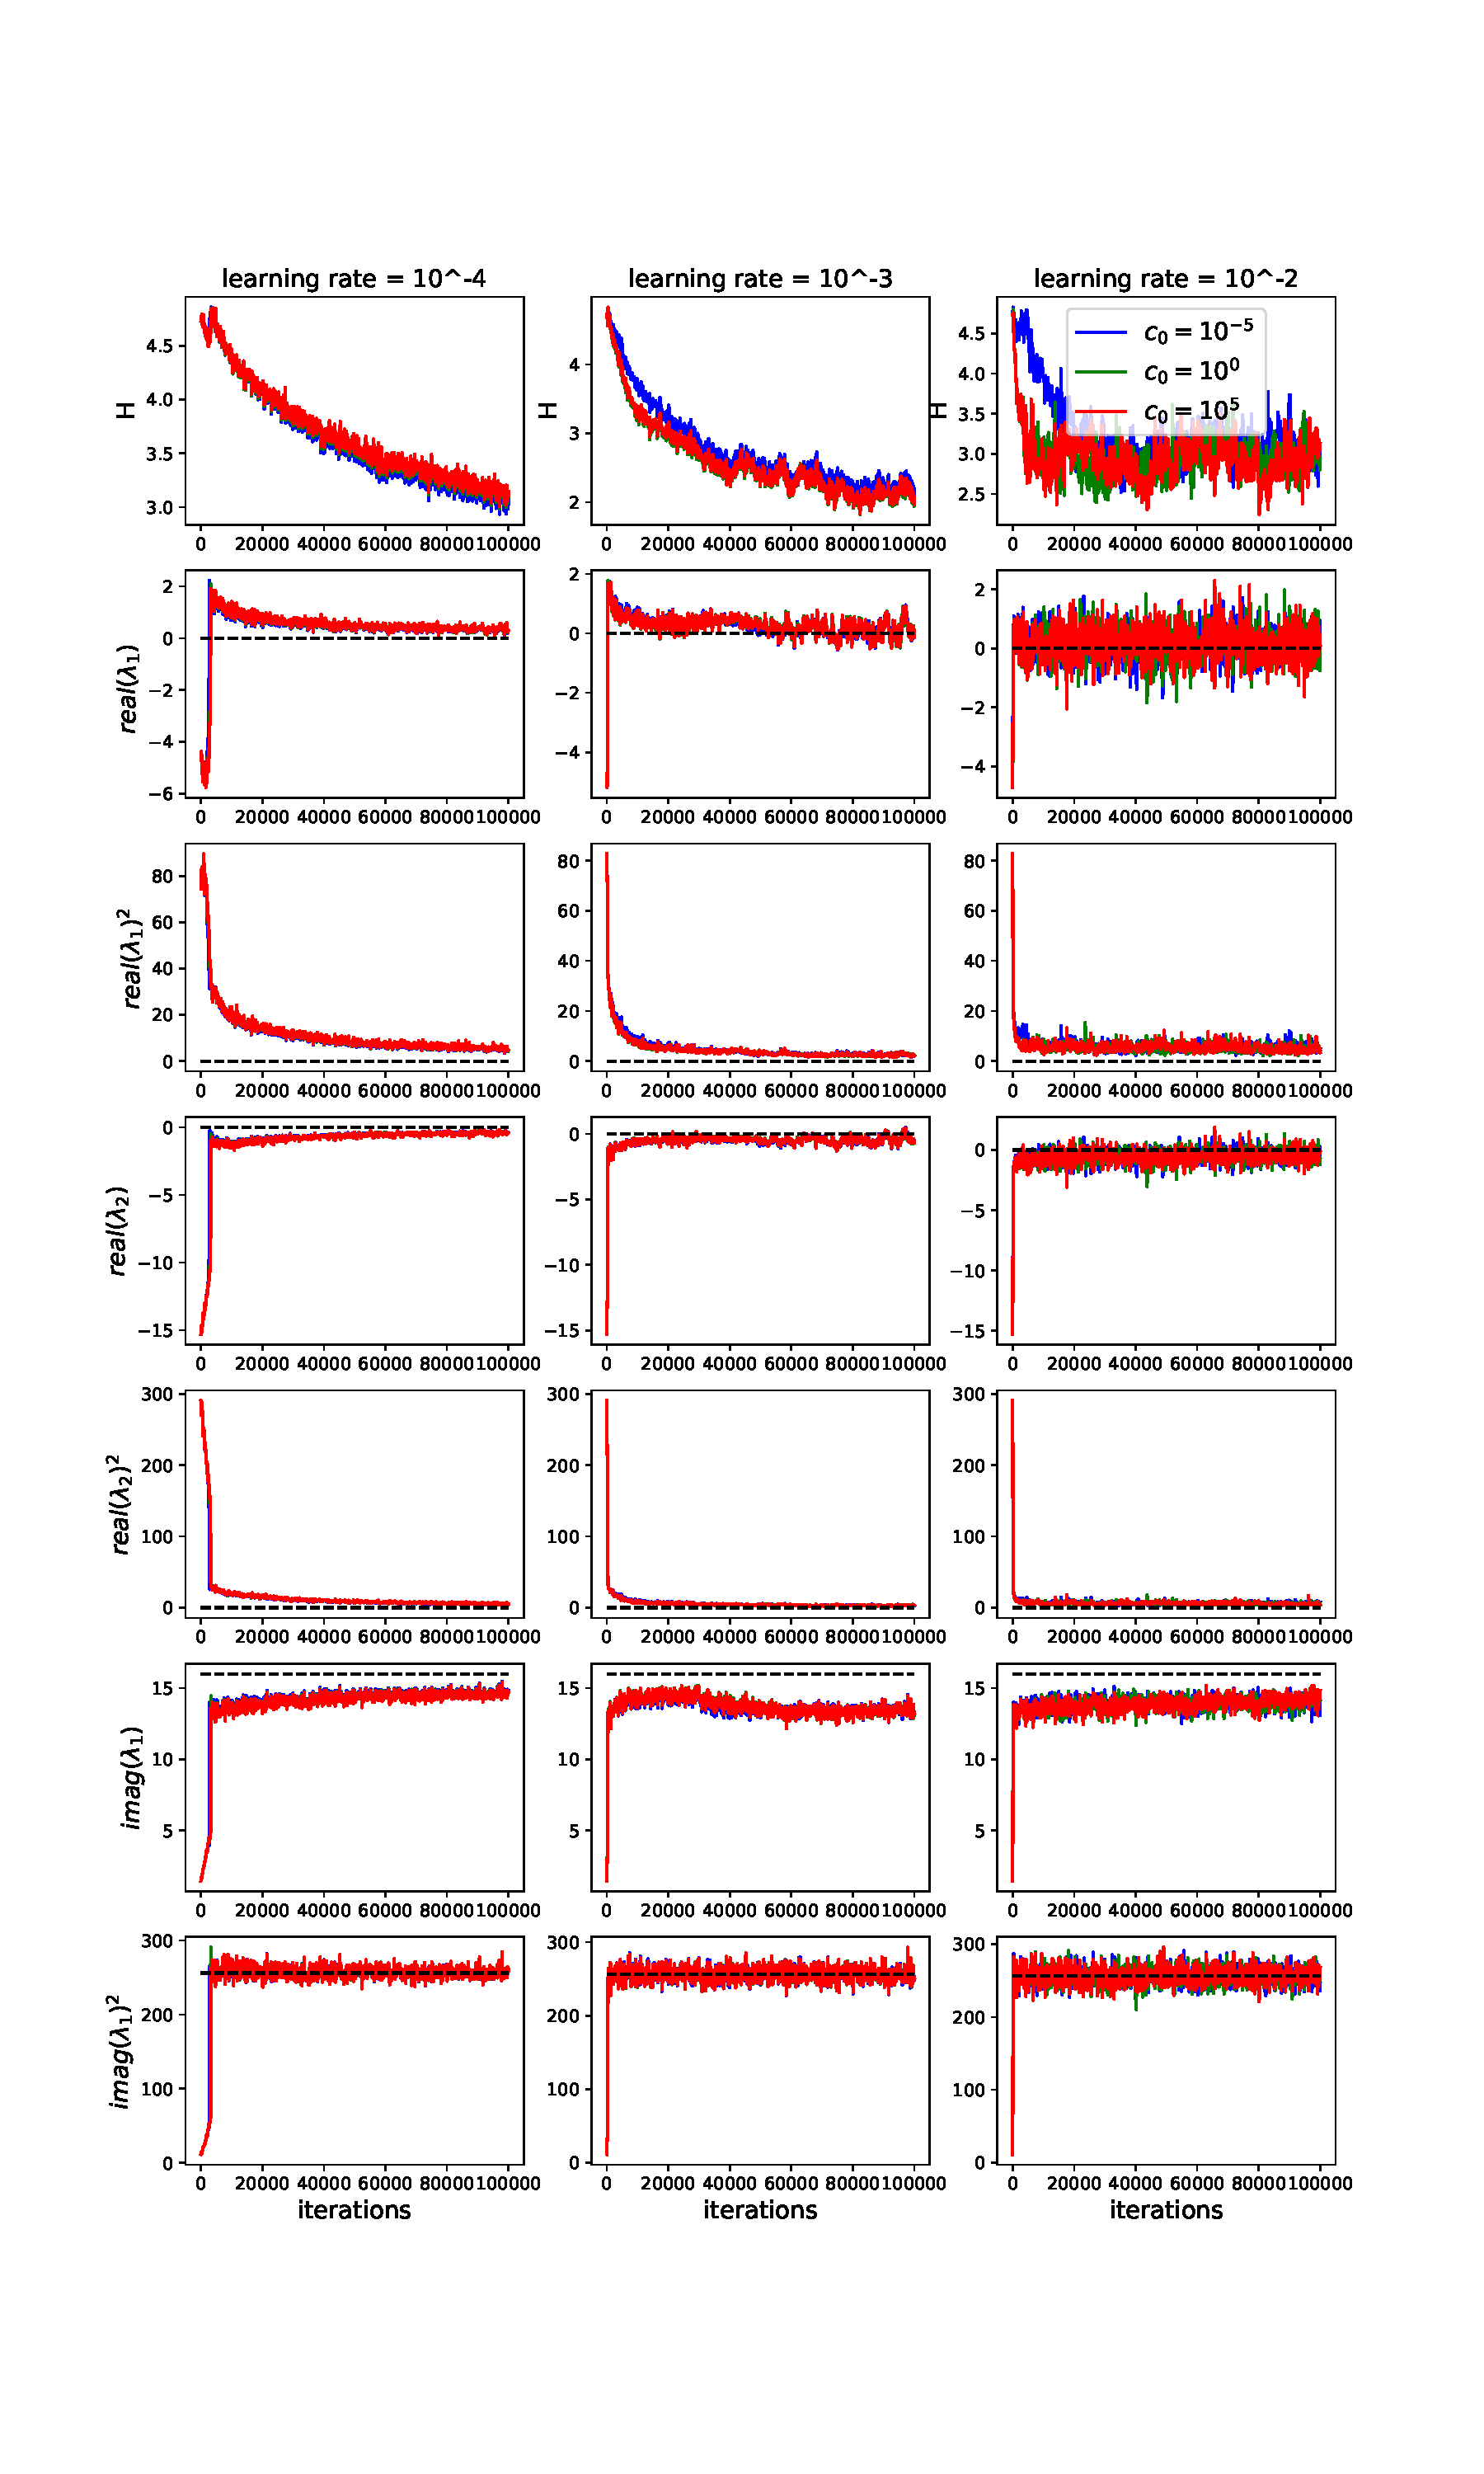
\includegraphics[scale=.45]{images/learnW_4P.pdf} \\
\end{center}

\clearpage
\begin{center}
\textbf{W: 8 planar layers} \\
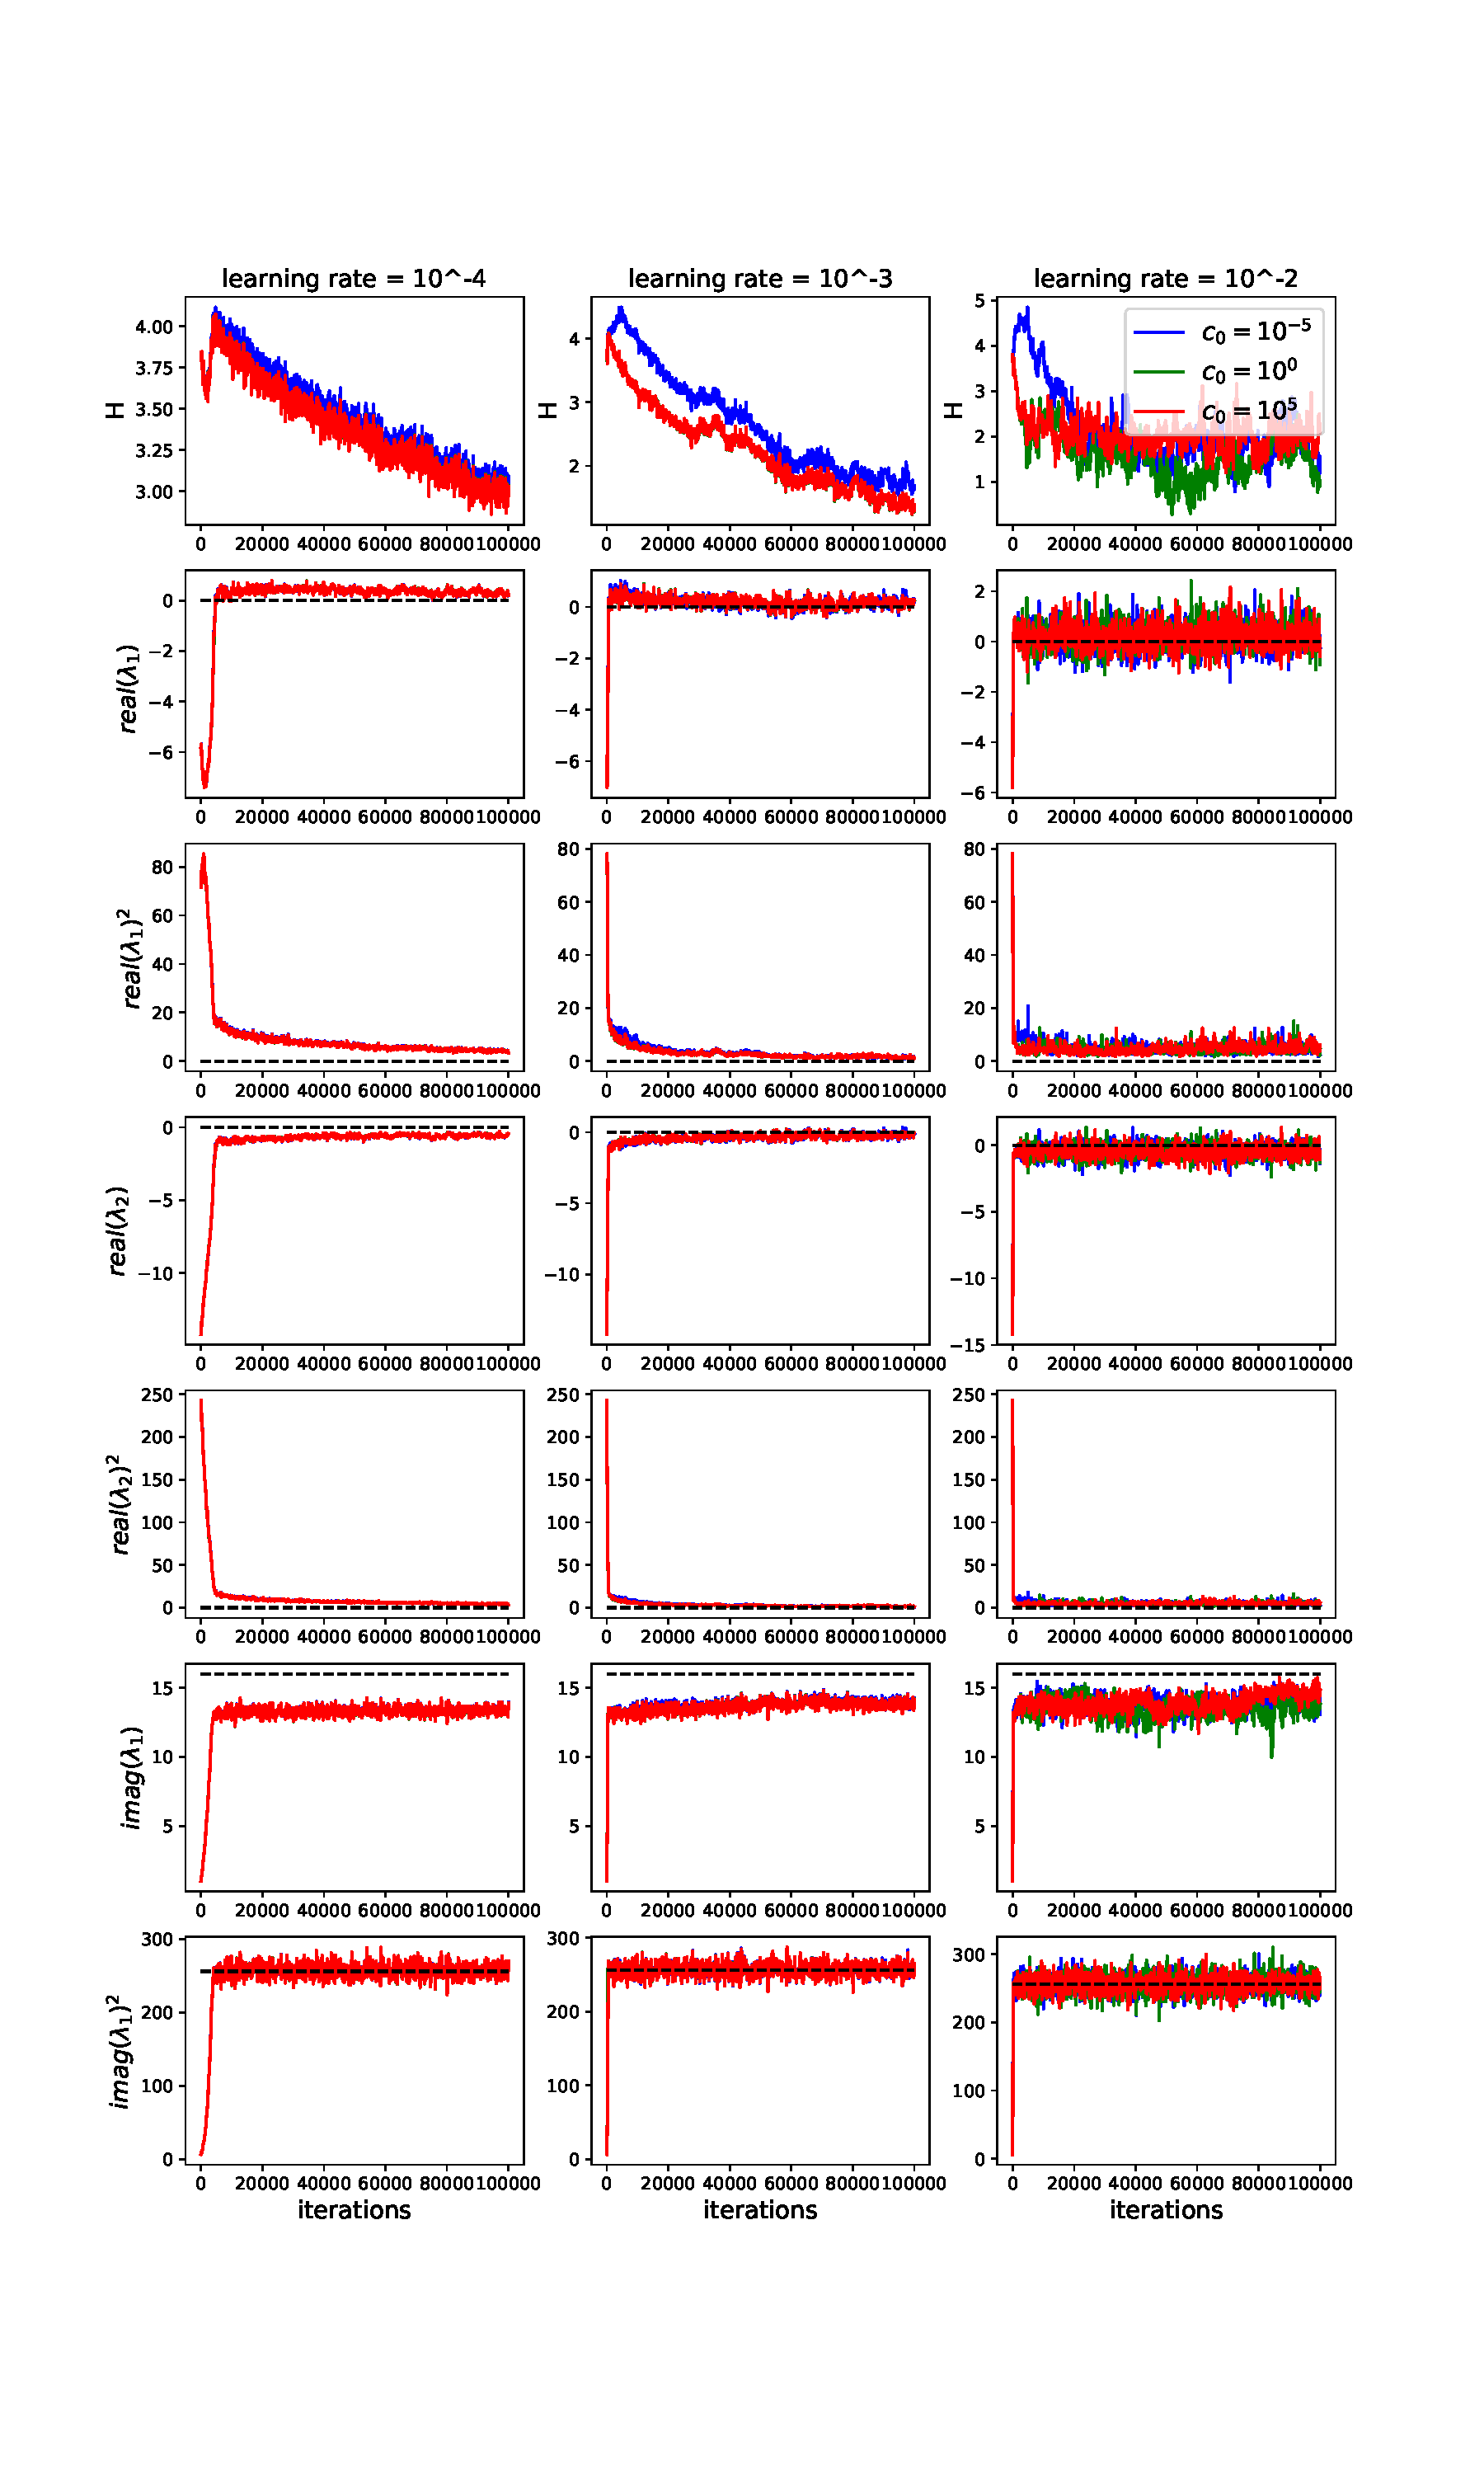
\includegraphics[scale=.45]{images/learnW_8P.pdf} \\
\end{center}

\clearpage
\begin{center}
\textbf{W: 10 planar layers} \\
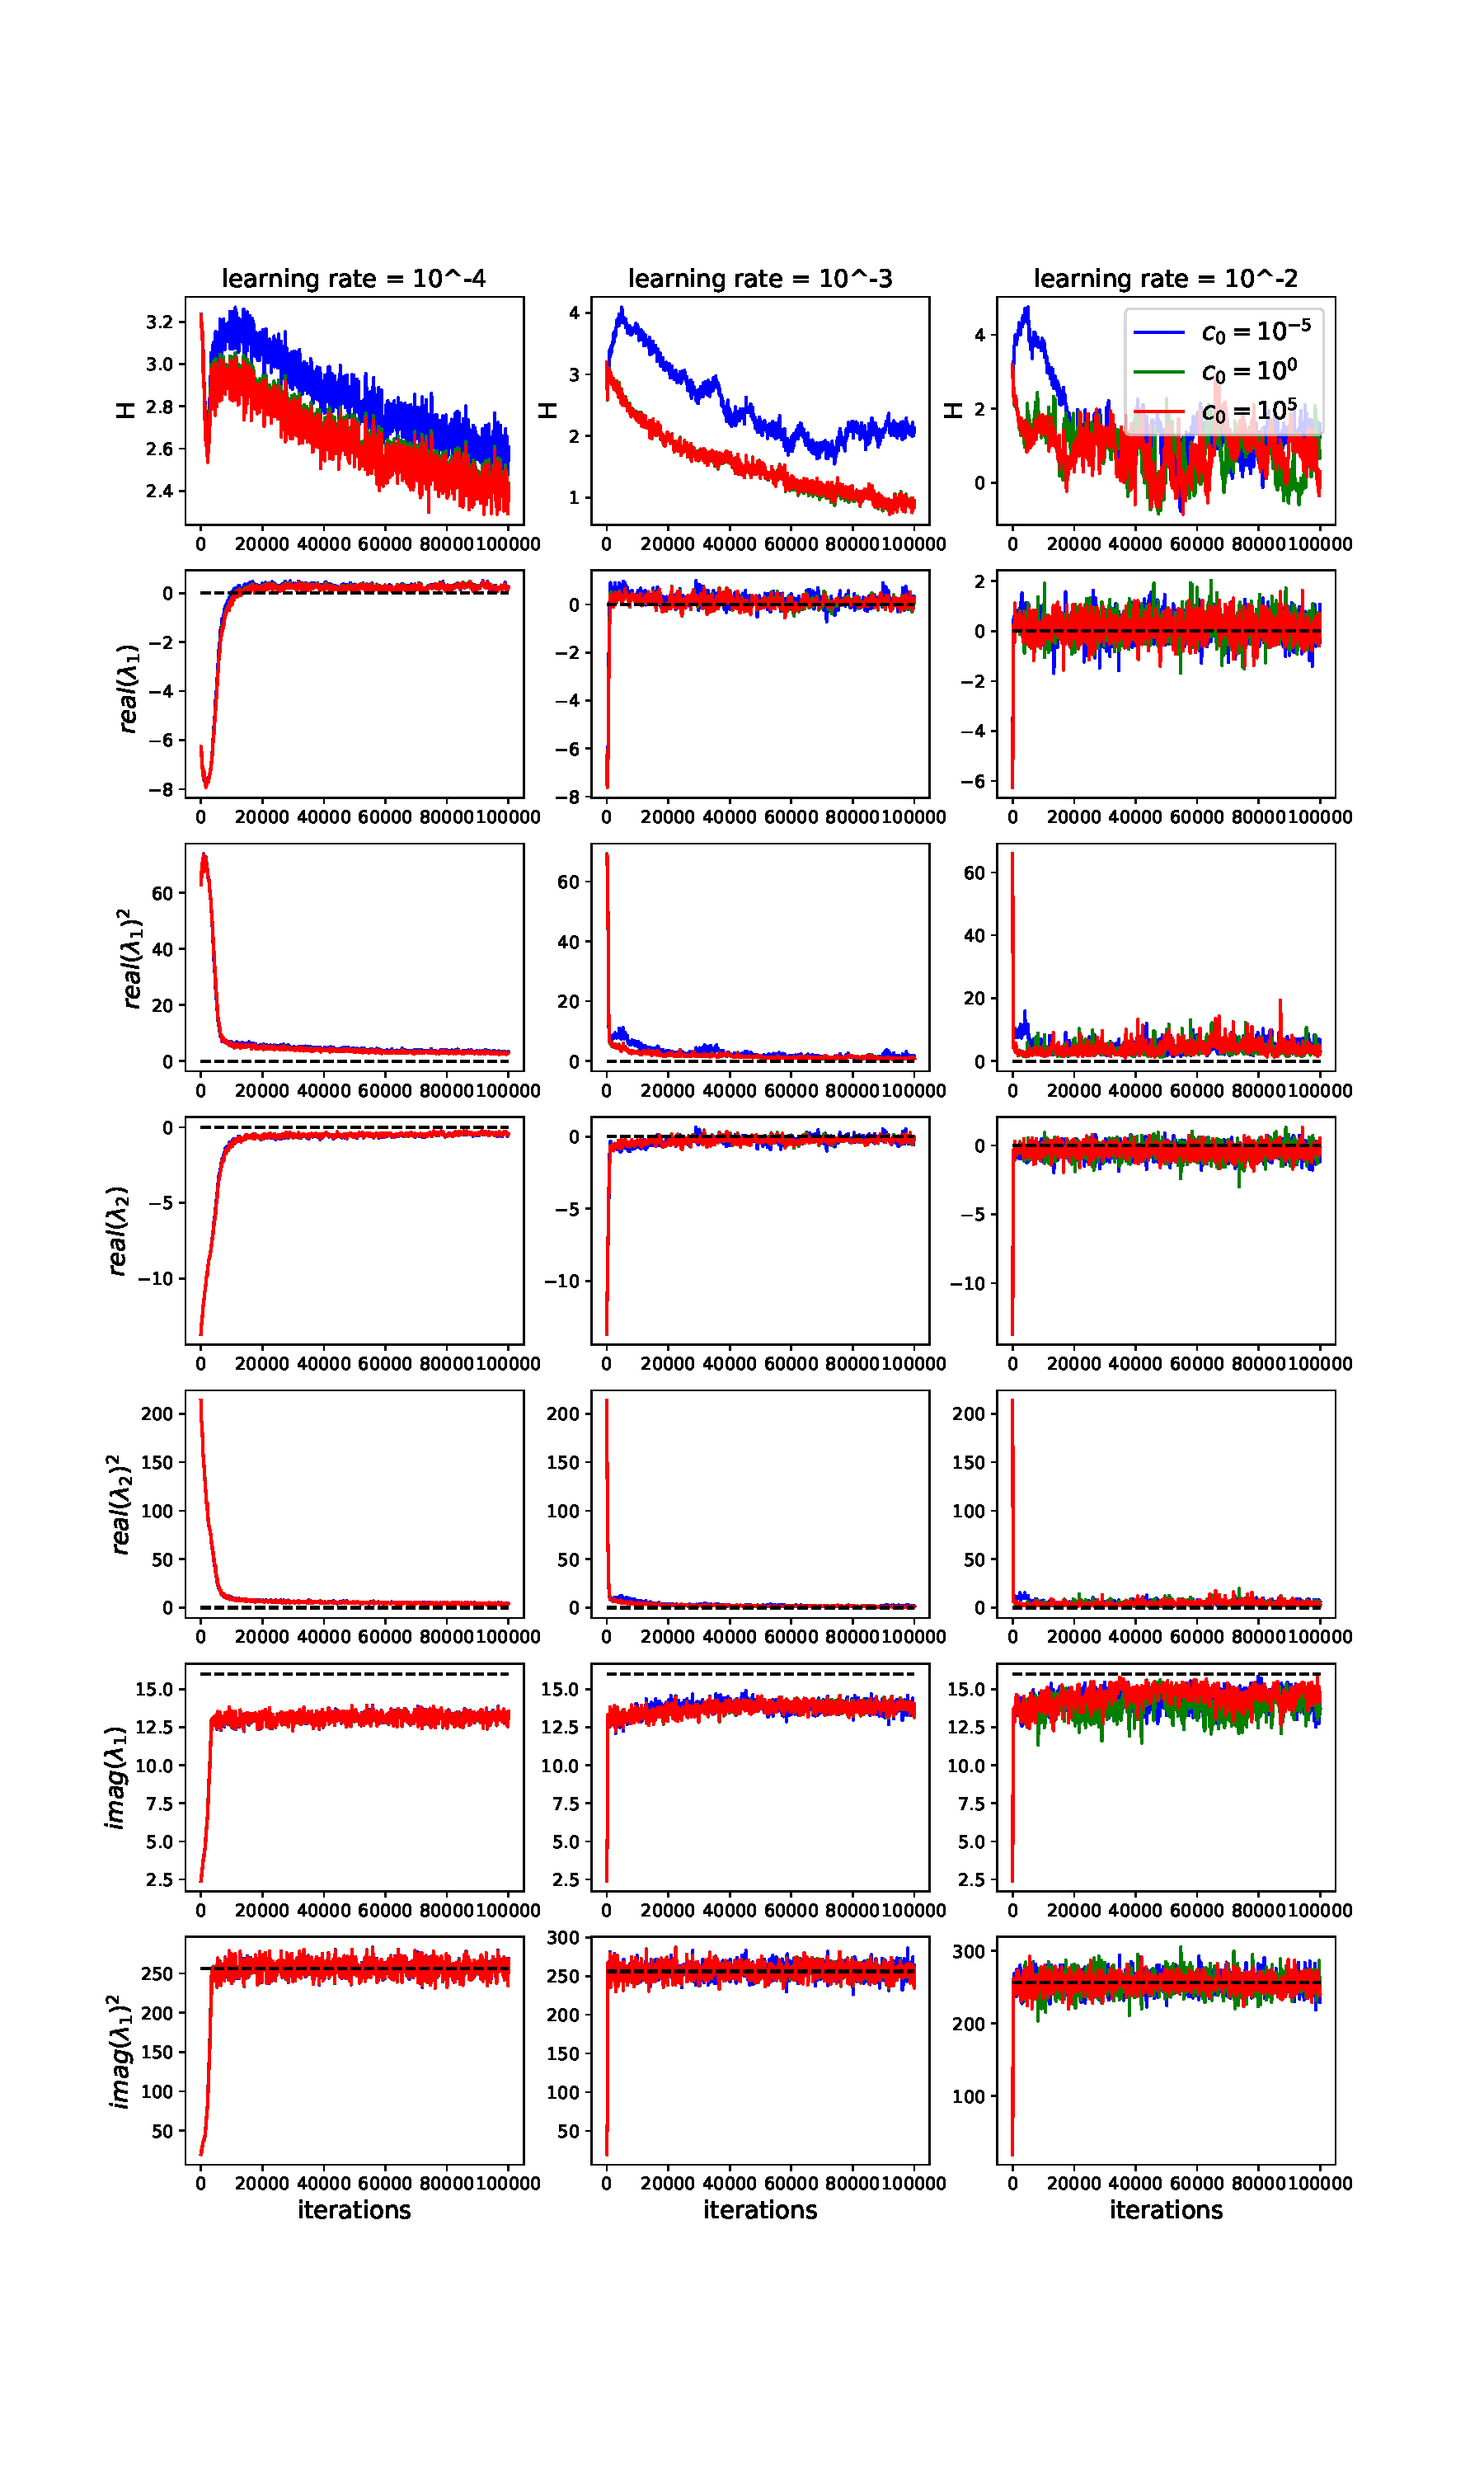
\includegraphics[scale=.45]{images/learnW_10P.pdf} \\
\end{center}

\clearpage
\begin{center}
\textbf{W: 10 planar layers}: $c_0 = 1$, learning rate = $10^{-3}$ \\
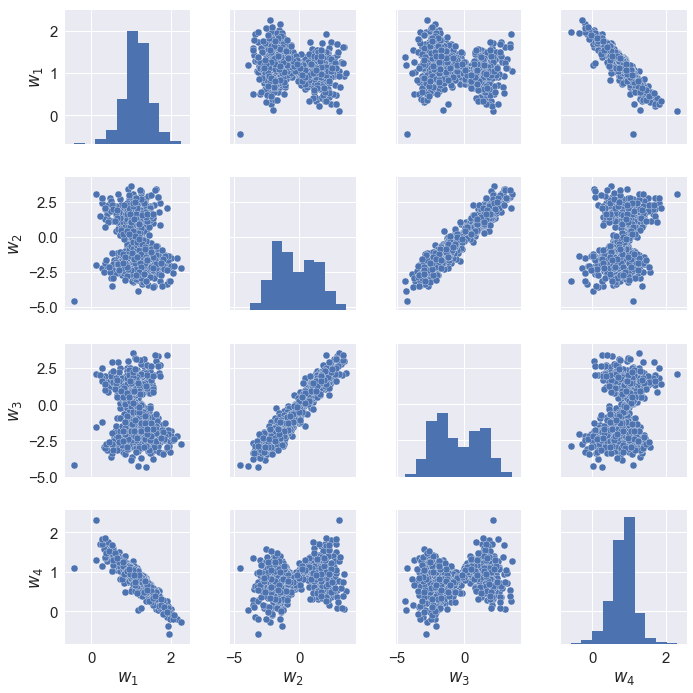
\includegraphics[scale=.45]{images/learnW_samples.png} \\
\end{center}




\end{document}

